\documentclass[enabledeprecatedfontcommands,fontsize=12.5pt,paper=a4,twoside]{scrartcl}


\newcommand{\grad}{\ensuremath{^{\circ}} }
\renewcommand{\strut}{\vrule width 0pt height5mm depth2mm}

\usepackage{longtable}
\usepackage[utf8]{inputenc}
\usepackage[T1]{fontenc}
\usepackage[final]{pdfpages}
% obere Seitenränder gestalten können
\usepackage{fancyhdr}
\usepackage{moreverb}
% Graphiken als jpg, png etc. einbinden können
\usepackage{graphicx}
\usepackage[normalem]{ulem}
\useunder{\uline}{\ul}{}
\usepackage{stmaryrd}
% Floats Objekte mit [H] festsetzen
\usepackage{float}
% setzt URL's schön mit \url{http://bla.laber.com/~mypage}
\usepackage{url}
% Externe PDF's einbinden können
\usepackage{pdflscape}
% Verweise innerhalb des Dokuments schick mit " ... auf Seite ... "
% automatisch versehen. Dazu \vref{labelname} benutzen
\usepackage[ngerman]{varioref}
\usepackage[ngerman]{babel}
\usepackage{ngerman}
% Bibliographie
\usepackage{bibgerm}
% Tabellen
\usepackage{tabularx}
\usepackage{supertabular}
\usepackage[colorlinks=true, pdfstartview=FitV, linkcolor=blue,
            citecolor=blue, urlcolor=blue, hyperfigures=true,
            pdftex=true]{hyperref}
\usepackage{bookmark}
\usepackage{rotating}
\usepackage{float}

\hyphenation{Arbeits-paket}

% Damit Latex nicht zu lange Zeilen produziert:
\sloppy
%Uneinheitlicher unterer Seitenrand:
%\raggedbottom

% Kein Erstzeileneinzug beim Absatzanfang
% Sieht aber nur gut aus, wenn man zwischen Absätzen viel Platz einbaut
\setlength{\parindent}{0ex}

% Abstand zwischen zwei Absätzen
\setlength{\parskip}{1ex}

% Seitenränder für Korrekturen verändern
\addtolength{\evensidemargin}{-1cm}
\addtolength{\oddsidemargin}{1cm}

\bibliographystyle{gerapali}

% Lustige Header auf den Seiten
  \pagestyle{fancy}
  \setlength{\headheight}{70.55003pt}
  \fancyhead{}
  \fancyhead[LO,RE]{Software--Projekt 2\\ WiSe 2019/2020
  \\Architekturbeschreibung}
  \fancyhead[LE,RO]{Seite \thepage\\\slshape \leftmark\\\slshape \rightmark}

%Unicode Minuszeichen deklarieren, um es nicht überall austauschen zu müssen
\DeclareUnicodeCharacter{2212}{-}

%
% Und jetzt geht das Dokument los....
%

\begin{document}

% Lustige Header nur auf dieser Seite
  \thispagestyle{fancy}
  \fancyhead[LO,RE]{ }
  \fancyhead[LE,RO]{Universität Bremen\\FB 3 -- Informatik\\
  Prof. Dr. Rainer Koschke \\TutorIn: Marcel Steinbeck}
  \fancyfoot[C]{}

% Start Titelseite
  \vspace{3cm}

  \begin{minipage}[H]{\textwidth}
  \begin{center}
  \bf
  \Large
  Software--Projekt 2 WiSe 2019/2020\\
  \smallskip
  \small
  VAK 03-BA-901.02\\
  \vspace{3cm}
  \end{center}
  \end{minipage}
  \begin{minipage}[H]{\textwidth}
  \begin{center}
  \vspace{1cm}
  \bf
  \Large Architekturbeschreibung\\
  \vfill
  \end{center}
  \end{minipage}
  \vfill
  \begin{minipage}[H]{\textwidth}
  \begin{center}
  \sf
  \begin{tabular}{lr}
  Liam Hurwitz & hurwitz@tzi.de \\
  Kevin Santiago Rodriguez Rey & kev\textunderscore rey@tzi.de \\
  Fabian Kehlenbeck & fkehlenb@tzi.de \\
  Aaron Rudkowski & rudkows@tzi.de \\
  Samuel Nejati Masouleh & samnej@tzi.de \\
  Leonard Haddad & s\textunderscore xsipo6@tzi.de \\  
\end{tabular}
  \\ ~
  \vspace{2cm}
  \\
  \it Abgabe: 22. Dezember 2019 --- Version 1.0\\ ~
  \end{center}
  \end{minipage}

% Ende Titelseite

% Start Leerseite

\newpage

  \thispagestyle{fancy}
  \fancyhead{}
  \fancyhead[LO,RE]{Software--Projekt \\  2019/2020
  \\Architekturbeschreibung}
  \fancyhead[LE,RO]{Seite \thepage\\\slshape \leftmark\\~}
  \fancyfoot{}
  \renewcommand{\headrulewidth}{0.4pt}
  \tableofcontents

\newpage

  \fancyhead[LE,RO]{Seite \thepage\\\slshape \leftmark\\\slshape \rightmark}


%%%%%%%%%%%%%%%%%%%%%%%%%%%%%%%%%%%%%%%%%%%%%%%%%%%%%%%%%%%%%%%%%%%%%%%%
\section*{Version und Änderungsgeschichte}

{\em Die aktuelle Versionsnummer des Dokumentes sollte eindeutig und gut zu
identifizieren sein, hier und optimalerweise auf dem Titelblatt.}

\begin{tabular}{ccl}
Version & Datum & Änderungen \\
\hline
0.1 & TT.MM.JJJJ & Dokumentvorlage als initiale Fassung kopiert \\
0.2 & 04.12.2019 & Faktortabelle \\
0.3 & 04.12.2019 & Problem Karten \\
\ldots
\end{tabular}


%%%%%%%%%%%%%%%%%%%%%%%%%%%%%%%%%%%%%%%%%%%%%%%%%%%%%%%%%%%%%%%%%%%%%%%%
\section{Einführung}

Diese Architektur Beschreibung wurde im Rahmen von Software Projekt 2 im Wintersemester 2019/2020 geschrieben. Das Projekt wurde im Rahmen des SFB 1232 Farbige Zustände erstellt. Die SFB-intitative \glqq Farbige Zustände\grqq{} erarbeitet sich eine neuartige experimentelle Methode der Werkstoffentwicklung.

Es handelt sich hierbei um eine Webapplikation, welche den Mitarbeitern der SFB-Initiative ermöglichen soll, effizient und ohne Verzögerung durch einen administrativen Mehraufwand Prozessketten für die untersuchten metallischen Konstruktionswerkstoffe zu finden. 
Außerdem ermöglichen wir es den Forschern der SFB-Initative den Überblick über laufende Prozessketten und deren ProzessSchritte zu behalten.
Konkret bedeutet dies, dass wir es den Logistikbeauftragten mithilfe unserer Software ermöglichen, Proben und deren Träger zu verwalten. Den Technologen der SFB-Initiative ermöglichen wir es, den Überblick über ihre Experimentierstationen zu behalten; sie werden immer über die laufenden ProzessSchritte informiert sein.
Dem Prozesskettenadministrator möchten wir es ermöglichen, Prozessketten zu erstellen und verwalten, welche auf digitalem Wege an die Technologen weitergegeben werden als auszuführende Aufträge, welche diese wiederum annehmen und durchführen können.
Außerdem möchten wir den Mitarbeitern im Lager ermöglichen, eine klare Übersicht über die im Lager sich befindende Proben zu behalten.
Außerdem möchten wir dem Transporter der Proben, welcher diese von A nach B transportieren muss, ermöglichen, diese Transporte einfach protokolliert durchführen zu können, mit einfachem Probenverlustprotokoll. 
Zu guter Letzt soll es noch dem System-Administrator möglich sein, die Benutzer des Systems zu verwalten und ihnen ihre Rollen im SFB zuzuteilen.
 
Diese Webapplikation soll also, in Stichpunkten, die folgenden Funktionen ermöglichen:
\begin{itemize}
  \item Die Erstellung und Verwaltung von Prozessketten durch einen Prozessketten-Administrator.
  \item Eine protokollierte, (digital semi-automatische-) beobachtete Durchführung von Experimenten auf die Werkstoff-Proben. 
  \item Ein protokollierter Transport der Proben in ihren Trägern von A nach B, mit Verlustprotokoll.
  \item Eine einfache Übersicht über die im Lager befindende Proben zu haben.
  \item Nutzer der Webapplikation einfach verwalten und ihren Rollen im SFB einteilen zu können.
  \item Das System sollte zudem auch noch lauffähig auf mobilen Geräten sein, und möchte noch auf Englisch verfügbar sein.
\end{itemize}

Leser dieser Architekturbeschreibung sind hiermit also nicht nur die Mitarbeiter der SFB-Initiative, sondern gegeben falls auch der Endkunde, welcher die Benutzer des Systems verwalten kann.

\subsection{Zweck}

  { Diese Architekturbeschreibung beschreibt die Architektur von Farbiges SFB, eine digitale Software welche die Erstellung, Verwaltung und Durchführung von Prozessketten ermöglicht, mit wessen Hilfe neue Werkstoffeigenschaften gefunden werden sollen für den industriellen Gebrauch. Es beschreibt, wie das System von Farbiges SFB implementiert werden soll und wie seine Struktur aussehen wird. 
Dieses Dokument soll allen, die die Software bedienen und bearbeiten werden, dabei helfen die Struktur und Funktionsweise von Farbiges SFB zu verstehen. Es soll sowohl den Entwicklern eine Übersicht über die Funktionsweise der Software geben, welche diese schließlich implementieren werden, als auch den Testern zur Vorbereitung ihrer Tests. Es soll außerdem dem Systemadministrator eine Übersicht der Software geben, da diese das System anschließend verwalten müssen und diese vielleicht die Software weiterentwickeln möchten. 
}

\subsection{Status}

{ Diese Architektur beschreibt den ersten Entwurf dieser Software. Es wurde auch noch nicht freigegeben durch ein Architekturreview, und ist somit die allererste Version.  }



\subsection{Definitionen, Akronyme und Abkürzungen}
In diesem Kapitel werden Akronyme und andere Ausdrücke definiert, welche im Laufe des Dokuments verwendet werden.

\begin{longtable}[c]{|p{7cm}|p{8cm}|}
\hline
\multicolumn{1}{|c|}{\textbf{Begriff}}                          & \multicolumn{1}{c|}{\textbf{Erklärung}}                                                                                                                                                                                                               \\ \hline
\endhead
%
\multicolumn{2}{|l|}{{\ul \textbf{Das System Selbst}}}                                                                                                                                                                                                                                                                  \\ \hline
Probe                                                           & Ein einzelner Werkstoff                                                                                                                                                                                                                              \\ \hline
Werkstoff                                                       & Mikrokugeln die sich durch Härte, hohe Belastbarkeit, Temperaturbeständigkeit und Abriebfestigkeit auszeichnen                                                                                                                                     \\ \hline
Träger                                                          & Transportmittel für Proben. Arten: Einzelträger, eingebettete Träger und Glasträger. Proben werden immer in Trägern transportiert                                                                                                                     \\ \hline
Experimentierstation \textbf{(ES)}             & Physischer Standort an dem Technologen Messungen durchführen.                                                                                                                                                                                     \\ \hline
Technologe                                                      & Ein Angestellter im SFB, er forscht und bedient die Experimentierstationen, und wertet diese im Anschluss aus und schreibt die Probeneigenschaften in die Software.                                                                                                  \\ \hline
Prozesskette \textbf{(PK)}                       & Besteht aus vielen ProzessSchritten, die hintereinander ohne Verzweigung ablaufen. Sobald ein Auftrag erfolgt, wird eine Prozesskette gestartet.                                                                                                        \\ \hline
Prozesskettenauftrag \textbf{(PK-Auftrag)}     & Enthält die Prozessparameter für jeden Schritt einer Prozesskette. Der Prozesskettenadministrator legt die Prozessparameter fest. Der Logistiker legt die Proben und Träger fest.                                                                     \\ \hline
ProzessSchritt \textbf{(PS)}                     & In einem ProzessSchritt werden Werkstoffeigenschaften beeinflusst und / oder verändert. Er enthält Prozessparameter, welche beschreiben wie die Eigenschaften beeinflusst werden. Ein ProzessSchritt kann Vorbedingungen haben und eine geschätzte Dauer. \\ \hline
Material- / Werkstoffeigenschaften                              & Jeder Werkstoff besitzt Eigenschaften. (Umformbarkeit / Verformbarkeit / ...)                                                                                                                                                                        \\ \hline
Prozessparameter \textbf{(PP)}                   & Sind qualitativ oder quantitativ. Qualitativ beschreibt, ob etwas so ist oder nicht. Quantitative Parameter enthalten einen Namen, ein Wert und eine Einheit.                                                                                          \\ \hline
Logistiker                                                      & Verwaltet das Archiv und alle Proben und Träger. Für die Ausführung einer Prozesskette bestimmt er welche Proben benutzt werden, falls dies nicht möglich ist, meldet er es dem Prozesskettenadministrator.                                           \\ \hline
Prozesskettenadministrator\textbf{ (PK-Admin)} & Verwaltet Prozessketten und deren ProzessSchritte nach bestimmten Vorlagen. Verwaltet auch die Vorlagen. Ordnet ProzessSchritten Experimentierstationen zu. Überprüft dann auf Korrektheit.                                                           \\ \hline
Transporter                                                     & Transportiert Träger mit ihren Proben zwischen Experimentierstationen. Bei Probenverlust meldet er diese.                                                                                                                                             \\ \hline
Transportauftrag \textbf{(T-Auftrag)}          & Enthält Start- und Zielexperimentierstationen, wird vom Transporter ausgeführt.                                                                                                                                                                      \\ \hline
System Administrator \textbf{(Sys-Admin)}      & Verwaltet Nutzer und Experimentierstationen. Konfiguriert globale Einstellungen und ist für Backups zuständig.                                                                                                                                         \\ \hline
Prozessketteninstanz Werte \textbf{(PIW)}      & Enthält für jeden ProzessSchritt der Prozesskette alle Prozessparameter. Der Prozesskettenadmin benutzt die PIWs um Prozessketteninstanzen zu planen.                                                                                                 \\ \hline
Standort                                                        & Träger und Proben können entweder an einer Experimentierstation, im Archiv oder als verloren gemeldet sein.                                                                                                                                           \\ \hline
Transportauftragzustand \textbf{(TA-Zustand)}  & Ein Transportauftrag befindet sich im Zustand wartend oder er wurde schon geliefert.                                                                                                                                                                  \\ \hline
ProzessSchrittzustand \textbf{(PS-Zustand)}    & Ein ProzessSchrittzustand hat entweder den Zustand angenommen, in Bearbeitung oder abgegeben.                                                                                                                                                         \\ \hline
Upload in Datenbank                                             & Ein Technologe muss nach dem Ausführen eines ProzessSchrittes die Prozessparameter in die Datenbank (DAVIS) hochladen.                                                                                                                                \\ \hline
\end{longtable}

\begin{longtable}[c]{|p{7cm}|p{8cm}|}
\hline
\multicolumn{1}{|c|}{\textbf{Begriff}} & \multicolumn{1}{c|}{\textbf{Erklärung}}                                                                                                                                                                                 \\ \hline
\endhead
%
\multicolumn{2}{|l|}{{\ul \textbf{Technische Ausdrücke}}}                                                                                                                                                                                                        \\ \hline
Anwendungsfälle                        & Hilfsmittel, um Anforderungen unseres Software-Projekts zu erfassen. Sie beschreiben also, was unser System tun soll. Hierzu nutzen wir Akteure und Use-Cases.                                                         \\ \hline
H2                                     & Eine SQL Java Datenbank, die auch die JDBC API unterstützt.                                                                                                                                                              \\ \hline
Apache Maven                           & Ist ein automatisches Buildtool für Java Projekte. Es beschreibt, wie Software gebaut wird und was ihre Dependencies sind.                                                                                              \\ \hline
DAO                                    & Objekte, die abstrakte Interfaces zu Datenbanken oder anderen Persistenzmechanismen bieten. Kurzgesagt, werden sie verwendet, um Daten aus einer Datenbank zu verwalten (Data Access Object).                             \\ \hline
Java                                   & Eine objektorientierte Programmiersprache, welche klassenbasiert ist. Läuft universell auf fast allen Platformen, die eine JVM haben, von PCs zu Handys usw...                                       \\ \hline
JavaEE (JakartaEE)                     & Ist eine Menge an Spezifikationen für Java SE welche Enterprise Features und Webservices sowie Distributed Computation spezifiziert.                                                                                    \\ \hline
Hibernate Validator                    &  \\ \hline
Lombok                                 & Ist eine Java Bibliothek welche zur automatisierten Code-Erstellung verwendet weden kann (um nicht so viel Code schreiben zu müssen) z. B. automatische Erstellung von Gettern und Settern, Equals, Hashcode und String. \\ \hline
JUnit                                  & Ist ein Unit Testing Framework für Java, zur Überprüfung von bekannten Fehlern in den implementierten Funktionen und Klassen.                                                                                          \\ \hline
Wildfly                                & Ist ein Application Server, der die JavaEE Spezifikation implementiert.                                                                                                                                                 \\ \hline
Mockito                                & Ist ein Mocking Framework für JUnit, zum weiteren Testen der implementierten Funktionen. Es ermöglicht die Erstellung von Test Double Objekte für automatische Unit Tests.                                              \\ \hline
Scrypt                                 & Eine passwortbasierte Schlüsselableitungsfunktion, die nicht umkehrbar ist.                                                                                                                                             \\ \hline
Bootsfaces                             & Ist eine JSF Framework, welche Bootstrap und JQuery benutzt, um responsive Front-Ends zu entwickeln.                                                                                                                      \\ \hline
Primefaces                             & Ist eine Menge an UI Komponenten für JSF. Es bietet Templates und Themes an.                                                                                                                                            \\ \hline
JSF                                    & Steht für Java Server Faces. Ist eine Spezifikation zur Entwicklung von grafischen Oberflächen in Java.                                                                                                                \\ \hline
GUI                                    & Eine Form eines User Interfaces, die dem Benutzer erlaubt durch elektronische Geräte grafisch mit der Software zu interagieren (Graphical User Interface).                                                         \\ \hline
Klassendiagramm                        & Ist ein Typ von statischen Struktur Diagrammen, welche Klassen, Attribute, Operationen und Relationen des Systems als Diagramm darstellen.                                                                              \\ \hline
Komponentendiagramm                    & Beschreiben wie Komponenten durch ihre Schnittstellen verbunden sind. Sie werden benutzt um die Struktur komplexer Systeme darzustellen.                                                                                \\ \hline
Model-View-Controller (MVC)            & Ein Architekturmuster welches für User Interfaces benutzt wird um Programmlogik in 3 Elemente zu unterteilen: Model, View und Controller.                                                                               \\ \hline
Object-Relation-Mapping (ORM)          & Ist ein Verfahren um Datentypen zwischen inkompatiblen Typ Systemen zu konvertieren. Dieses erstellt eine virtuelle Objekt Datenbank                                                                                                                                                                                                             \\ \hline
Packetdiagramm                         & Zeigt die Abhängigkeiten der Packete des Models.                                                                                                                                                                        \\ \hline
Sequenzdiagramme                       & Zeigt die Struktur unseres Models und stellt den Austausch von nachricten zwischen Objekten dar. Dabei wird eine Lebenslinie benutzt.                                                                                   \\ \hline
Problemkarten                          & Beschreiben Probleme und passende Strategien.                                                                                                                                                                           \\ \hline
SQL                                    & Ist eine domänenspezifische Sprache, die in der Softwareentwicklung benutzt wird und Daten in relationalen Datenbanken verwaltet.                                                                                         \\ \hline
\end{longtable}
\subsection{Referenzen}
\begin{itemize}
  \item Architekturbeschreibung von RainersRaiders im Rahmen von Softwareprojekt 2 - 2016
  \item Kickoff Folien
\end{itemize}
\subsection{Übersicht über das Dokument}

{  Im Kapitel 2 werden wir zunächst verschiedene Anwendungsfälle unserer Software beschreiben, welche wir als Ausgangspunkt für unsere Architekturstruktur verwenden werden. In Kapitel 3 werden die Einflussfaktoren, Probleme und Strategien, die zum Lösen der Probleme entworfen wurden, dargestellt.
In den Kapiteln 4, 5 und 7 werden die verschiedenen Sichten von Hofmeister gezeigt. Die Codesicht wird in diesem Projekt nicht behandelt.
Im nachfolgenden Kapitel 4 wird die konzeptionelle Sicht unserer Software beschrieben. In Kapitel 5 wird die Modulsicht und in Kapitel 7 wird die Ausführungssicht gezeigt. Kapitel 6 ist eine nähere Beschreibung der Architektursicht und wird durch ein Modell in der Datensicht dargestellt.
Im Kapitel 8 werden einige Anwendungsfälle dargestellt. Im abschließenden Kapitel 9 wird auf die mögliche zukünftige Entwicklung der Software bei neu eingehenden Wünschen der Kunden eingegangen.

}


%%%%%%%%%%%%%%%%%%%%%%%%%%%%%%%%%%%%%%%%%%%%%%%%%%%%%%%%%%%%%%%%%%%%%%%

\section{Anwendungsfälle}

In diesen Kapitel werden wir verschiedene Anwendungsszenarien abdecken, welche unsere Software erfüllen soll. Diese Szenarien werden wir als Ausgangs- und Vergleichspunkt für den Rest unserer Architektur benutzen. Hiermit kann am Ende geprüft werden, ob die Software alle Anforderungen erfüllt. 

\textbf{•}\subsection{Anmeldung am System (alle Benutzer)}

Der Benutzer wird mit einem Login-Fenster begrüßt an welchem er sich einloggen kann. Sollte es noch keinen Benutzer im System geben, so kann ein neuer Benutzer über ein Create-Account Knopf erstellt werden. Sollte er sein Passwort vergessen haben, so kann er mithilfe von einem Passwort Vergessen Knopf dieses zurücksetzen.
Nach der Erstellung eines Benutzers wird dieser im Datenbanksystem eingespeichert, wodurch der System Administrator ihm nun eine Rolle einteilen kann.
Der System Administrator befindet sich schon zu Anfang im System. Das heißt er muss seinen Benutzer nicht neu erstellen.
Nach einer erfolgreichen Anmeldung am System werden alle Benutzer mit einer Navigationstabelle begrüßt. Diese Tabelle beinhaltet die für den Benutzer spezifizierten Funktionalitäten.

\subsection{Benutzer Verwaltung - System Administrator}

Die Aufgabe des System Administrators ist es die Benutzer zu verwalten. Nach seiner Anmeldung am System wird dieser mit einer Tabelle begrüßt welche seine Optionen im System anzeigt. Nach druck auf den Knopf für Nutzerverwaltung wird er mit einer weiteren Tabelle begrüßt, welche alle Nutzer des Systems beinhaltet. Diese Tabelle hat sowohl einen sortierungs Knopf, als auch eine Suchbox, wodurch er die angezeigten Nutzer des Systems filtern kann.
Jeder Nutzer hat einen Bearbeitungsknopf neben seinem Namen. Durch druck auf diesen Knopf öffnet sich ein weiteres Fenster, in dem der Systemadministrator alle Optionen zur Verwaltung des Nutzers hat. Hier kann er z.B. dessen Details ändern (Name, Vorname, usw...), seine Rolle im SFB (Technologe, Transporter, usw...), aber auch einen Löschung Knopf mit welchem er diesen Benutzer aus dem System entfernen kann. 
Die Tabelle beinhaltet natürlich auch einen Add Knopf, wodurch der System Administrator neue Benutzer im System einfügen kann. 

\subsection{Experimentierstationsverwaltung - System Administrator}

Wir nehmen an der Administrator hätte sich schon im System angemeldet. In dem vor ihm stehendes Fenster sieht er unter der Benutzerverwaltung einen weiteren Knopf zur Experimentierstationsverwaltung. Durch druck auf diesen Knopf öffnet sich ein weiteres Fenster mit einer weiteren Tabelle welche alle im System enthaltenden Experimentierstationen beinhaltet.  Diese sind auch wieder mal in reihen der Tabelle eingeteilt. Jede Reihe hat rechts einen Knopf mit welchem der Administrator die zugehörige Experimentierstation verwalten kann, und daneben einen weiteren Knopf zur Löschung der Experimentierstation.
Unten in der Tabelle befindet sich ein weiterer Knopf mit welchem er weitere Experimentierstationen einfügen kann.
Bei normalen druck auf eine Experimentierstation werden Informationen über diese angezeigt, wie z.B. Standort und ob diese momentan in Benutzung ist. 
  
\subsection{Prozesskettenverwaltung - Prozesskettenadministrator}

Da die Aufgabe des Prozesskettenadministrators die Erstellung und Verwaltung von Prozessketten ist, wird dieser nach seiner Anmeldung am System mit einem Fenster begrüßt, wo er durch druck auf den Knopf zur Prozesskettenverwaltung mit einem weiteren Fenster begrüßt wird, welches alle Prozessketten des Systems enthält.
Auch diese Tabelle kann durch eine Suchbox und weitere Kriterien wie z.B. Datum der Erstellung der Prozesskette filtriert werden.
In dieser Tabelle sind alle Prozessketten die sich im System befinden, in reihen sortiert, sichtbar. An der Seite jeder noch nicht instanziierten Prozesskette ist ein Knopf um diese zu Bearbeiten. Durch druck auf den Bearbeitungsknopf kann der Prozesskettenadministrator die Schritte dieser Prozesskette bearbeiten. Hier kann er z.B. weitere Schritte der Prozesskette hinzufügen, oder schon existierende Schritte entfernen.
Ein weiterer Knopf in der Tabelle erlaubt ihm eine Prozesskette zu starten. Sobald dieses getan ist, kann diese nicht mehr von ihm gestoppt werden.
Die Tabelle beinhaltet auch einen Einfügungs-Knopf, durch welchen weitere Prozessketten erstellt werden können.
Bei Erstellung einer Prozesskette wird diese auf Korrektheit überprüft. Sollte ein ProzessSchritt z.B. unrealistische Vorbedingungen haben, so wird dem Prozesskettenadministrator Bescheid gegeben, dass er diese Prozesskette im jetzigen Stand nicht erstellen kann.
Bei der Erstellung von Prozessketten, welche aus verschiedenen ProzessSchritten besteht, muss der Prozesskettenadministrator natürlich auch diese ProzessSchritte erstellen. Bei der Erstellung von Prozessketten wird er also mit einem Fenster begrüßt in welchem er die ProzessSchritte der Prozesskette verwalten kann.
Hier kann er z.B. einem ProzessSchritt Vorbedingungen geben, welche er in einem Vorbedingungsfeld eingeben kann. In einem weiteren Feld kann er die Experimentierstation dieses Schrittes zuordnen. Diese ProzessSchritte kann er so lange noch bearbeiten und verändern, bis die Prozesskette gestartet wird, durch den druck auf den Knopf zur Bearbeitung der Prozesskette.
Sollte eine Prozesskette in Bearbeitung sein, so kann der Prozesskettenadministrator auf diese drücken um zu sehen bei welchem Schritt sie sich momentan befindet. Er kann außerdem auch alle schon abgelaufenen- und noch auszuführende-Schritte sehen.
 
\subsection{Lagerübersicht - Logistiker}

Nehmen wir an der Logistiker hätte sich im System schon angemeldet.
In dem von ihm befindenden Fenster ist ein Knopf für Lagerübersicht. Durch druck auf diesen öffnet sich ein weiteres Fenster mit einer Tabelle welche alle sich im Lager befindenden Proben beinhaltet. Auch diese Tabelle kann durch Suchbox und weiteres filtriert werden. Sie beinhaltet aber auch eine Option zur Gruppierung der Proben nach Legierung, Wärmebehandlung und Stationen.

\subsection{Proben mit Prozessketten assoziieren - Logistiker}

Nach seinem Login findet der Logistiker in dem Begrüßungsfenster ein weiteren Knopf für Prozessketten. Hier kann er die verschiedenen Prozessketten sehen welche gerade ausgeführt werden und welche Proben sie benötigen. Durch eine schnelle suche mit z.B. der Suchbox im Lagerübersichtsfenster kann der Logistiker herausfinden, ob die benötigten Proben sich im Lager befinden. Es soll bei jeder Prozesskette auch einen automatisierten Suchknopf geben welcher diese Proben automatisch im Lager sucht.
Befinden sich die Proben im Lager, so kann er die Proben der Prozesskette zuweisen. Sollte das nicht der Fall sein, so kann er auf einen Knopf neben der Prozesskette drücken, wodurch dem Prozesskettenadministrator Bescheid gegeben wird das die benötigten Proben nicht verfügbar sind.
 
\subsection{Prozessketten Starten/Stoppen - Logistiker}

Sollten die benötigten Proben vom Letzten Absatz sich im Lager befinden, so kann der Logistiker durch einen weiteren Knopf eine noch nicht gestartete Prozesskette starten.
Sollte aus welchem Grund auch immer eine Prozesskette gestoppt werden, so kann dieser auch diese stoppen.

\subsection{Zustand eines Auftrags angeben - Technologe}

Nehmen wir an der Technologe hätte sich schon im System angemeldet. Er sieht vor sich ein Fenster mit einem Knopf für Aufträge. Durch druck auf diesen gelangt er zu einem weiteren Fenster in dem alle verfügbaren Aufträge als Reihen in einer Tabelle angezeigt werden. Hier kann er nun einen Auftrag annehmen, durch druck auf einen Knopf neben einem Auftrag, wodurch dieser Auftrag automatisch in den Zustand angenommen geht. Dieser Auftrag kann nun von keinem anderen Technologen mehr angenommen werden. Sobald der Technologe mit der Bearbeitung des Auftrags beginnt, muss er nur auf den Knopf für in-Bearbeitung drücken, wodurch dieser Auftrag nun automatisch in den Zustand in-Bearbeitung gelangt. Sobald der Technologe mit seiner Bearbeitung fertig ist, muss er nur auf einen Knopf drücken, wodurch der Auftrag nun als Bearbeitet gekennzeichnet wird. Sollte er nun diesen Auftrag weiterschicken möchten, so kann er dieses durch druck auf einen weiteren Knopf tun. Sobald der Technologe die Prozessparameter dieses Auftrags in der Datenbank hochgeladen hat, wird der Auftrag entweder automatisch auf in die DB hochgeladen gesetzt, oder manuell durch den Technologen. Dieses kommt drauf an ob der Technologe zum Hochladen der Daten den Knopf in diesem Auftrag verwendet hat, oder einen anderen.

\subsection{Aufnahme der Zeit in einem Auftrag - Technologe}

Bei der Annahme eines Auftrags aus dem  vorherigen Absatz wird die jetzige Systemzeit aufgenommen und im Auftrag eingegeben. Das gleiche passiert auch bei den weiteren Schritten aus dem vorherigen Absatz.
Sollte der Technologe allerdings an einem späteren Zeitpunkt diese Zeiten bearbeiten möchten, so kann er durch druck auf einen Bearbeitungsknopf neben dem Auftrag in der Tabelle die Zeiten manuell ändern.  

\subsection{Station Fehler Melden - Technologe}

Sollte irgendetwas schiefgehen und eine Station fehlerhaft werden, so kann der Technologe, nach seiner Anmeldung im System, durch einen Knopf einen Station Fehler melden. Hierdurch wird das System auch die Fehlernachricht bekommen, und somit allen anderen Prozessketten welche diese Station benötigen darüber Bescheid geben. 

\subsection{Proben Transportieren - Transporter}

Nehmen wir an der Transporter hätte sich schon am System angemeldet. Er sieht ein Fenster mit einem Transportübersicht Knopf, welcher ein weiteres Fenster öffnet, mit allen Transportaufträgen als Reihen in einer Tabelle. Hier kann er, durch druck auf einen Auftrag sehen, wo diese Proben abgeholt werden müssen, und wo sie hin geliefert werden müssen. 
Er kann durch Knopfdruck einen Auftrag annehmen, wodurch dieser als Annahme gekennzeichnet wird. Sobald er die Proben abgeholt hat, kann er durch Knopfdruck diesen Auftrag auf die Kennzeichnung Transport setzen. Sobald er die Proben zum korrekten Ort gebracht hat, kann er durch einen weiteren Knopfdruck diesen Auftrag als Ausgeliefert markieren.

\subsection{Probenverlust Melden - Transporter}

Nachdem der Transporter den Transport aus dem vorherigen Abschnitt ausgeführt hat, kann er durch druck auf einen Knopf innerhalb der Auftragstabelle für jeden Auftrag Probenverlust angeben. Hierdurch wird der Auftrag automatisch auf den Zustand Verlust gesetzt.


\section{Globale Analyse}

\label{sec:globale_analyse}

{\it Hier werden Einflussfaktoren aufgezählt und bewertet sowie Strategien
zum Umgang mit interferierenden Einflussfaktoren entwickelt.}

%%%%%%%%%%%%%%%%%%%%%%%%%%%%%%%%%%%%%%%%%%%%
\subsection{Einflussfaktoren}


%\label{sec:einflussfaktoren}
%{\it Hier sind Einflussfaktoren gefragt, die sich auf die Architektur
 % beziehen. Es sind ausschließlich architekturrelevante
 % Einflussfaktoren, und nicht z.\,B.\ solche, die lediglich einen
 % Einfluss auf das Projektmanagement haben. Fragt Euch also bei jedem
 % Faktor: Beeinflusst er wirklich die Architektur? Macht einen
 % einfachen Test: Wie würde die Architektur aussehen, wenn ihr den
 % Einflussfaktor E berücksichtigt? Wie würde sie aussehen, wenn Ihr E nicht
 % berücksichtigt? Kommt in beiden Fällen dieselbe Architektur heraus,
 % dann kann der Einflussfaktor nicht architekturrelevant sein.

  %Es geht hier um Einflussfaktoren, die
  %\begin{enumerate}
  %\item sich über die Zeit ändern,
  %\item viele Komponenten betreffen,
  %\item schwer zu erfüllen sind oder
  %\item mit denen man wenig Erfahrung hat.
  %\end{enumerate}
  %Die Flexibilität und Veränderlichkeit müssen ebenfalls charakterisiert werden.
  %\begin{enumerate}
  %\item Flexibilität: Könnt Ihr den Faktor zum jetzigen Zeitpunkt beeinflussen?
  %\item Veränderlichkeit: ändert der Faktor sich später durch äußere Einflüsse?
%\end{enumerate}

  %Unter Auswirkungen sollte dann beschrieben werden, {\em wie} der
  %Faktor {\em was} beeinflusst. Das können sein:
  %\begin{itemize}
  %\item andere Faktoren
  %\item Komponenten
  %\item Operationsmodi
  %\item Designentscheidungen (Strategien)
  %\end{itemize}

  %Verwendet eine eindeutige Nummerierung der Faktoren, um sie auf den
  %Problemkarten einfach referenzieren zu können.  }
  %%%%%%%%%%%%%%%%%%
die Notation der Flexibilität hat die  Bedeutung :
\begin{itemize}
    \item - - : Keine Flexibilität
    \item - : schlechte, aber nicht komplett starre Flexibilität
    \item ++: sehr gute Flexibilität
    \item +: gute Flexibilität
      Anforderungen.
  \end{itemize} 

\begin{table}[H]
\centering
\begin{tabular}{|p{1cm}|p{3cm}|p{5cm}|p{1cm}|p{5cm}|}
\hline
\begin{tabular}[c]{@{}l@{}}Abge-\\ leitet\\aus\end{tabular} & Einflussfaktor                                                                        & \begin{tabular}[c]{@{}l@{}}Flexibilität und \\ Veränderlichkeit\end{tabular}                                                              & \begin{tabular}[c]{@{}l@{}}++/\\\\ - -\end{tabular} & Auswirkungen                                                                                                                                                                                                                              \\ \hline
\multicolumn{5}{|l|}{O1 : Organisation}                                                                                                                                                                                                                                                                                                                                                                                                                                                                                                                                                          \\ \hline
\multicolumn{5}{|l|}{O1.1 Time-To-Market}                                                                                                                                                                                                                                                                                                                                                                                                                                                                                                                                                        \\ \hline
                                                          & \begin{tabular}[c]{@{}l@{}}Die Auslieferung\\  erfolgt am\\  08.03.2020.\end{tabular} & \begin{tabular}[c]{@{}l@{}}Keine\\ Veränderlichkeit oder \\Flexibilität, da Teil der\\ Mindestanforderungen.\end{tabular} & \begin{tabular}[c]{@{}l@{}}- -/\\   - -\end{tabular} & \begin{tabular}[c]{@{}l@{}}Nicht alle\\  Funktionen können\\  realisiert werden.\end{tabular}                                                                                                                                             \\ \hline
\multicolumn{5}{|l|}{O1.2 Architektur-Abgabe}                                                                                                                                                                                                                                                                                                                                                                                                                                                                                                                                                    \\ \hline
                                                          & \begin{tabular}[c]{@{}l@{}}Die Auslieferung \\erfolgt am\\ 22.12.2020.\end{tabular}      & \begin{tabular}[c]{@{}l@{}}Keine\\ Veränderlichkeit oder \\Flexibilität, da Teil der\\ Mindestanforderungen.\end{tabular} & \begin{tabular}[c]{@{}l@{}}- -/\\   - -\end{tabular} & \begin{tabular}[c]{@{}l@{}}Durch den\\ Zeitdruck könnte\\ die Architektur\\ mangelhaft\\ werden. Wenn wir\\ uns nicht genug\\ Zeit lassen,\\ könnten Aspekte,\\ die relevant für die\\ Architektur sind,\\ vergessen werden.\end{tabular} \\ \hline
\multicolumn{5}{|l|}{O1.3 Entwickler}                                                                                                                                                                                                                                                                                                                                                                                                                                                                                                                                                    \\ \hline
                                                          & \begin{tabular}[c]{@{}l@{}}Die\\ Projektgruppe \\besteht aus\\ 6 Entwicklern\\\end{tabular}      & \begin{tabular}[c]{@{}l@{}}Ein wenig Veränderlichkeit\\ und Flexibilität: \\Gruppenmitglieder könnten\\ die Gruppe verlassen.\end{tabular} & \begin{tabular}[c]{@{}l@{}}o/\\   o\end{tabular} & \begin{tabular}[c]{@{}l@{}} Die Architektur kann \\wegen Zeitmangel (es \\können nicht mehr \\als die ursprünglichen\\ sechs Entwickler mitarbeiten) \\und fehlenden Fähigkeiten\\ Mangel enthalten. \end{tabular} \\ \hline

\multicolumn{5}{|l|}{O1.4 Fähigkeiten Entwickler}                                                                                                                                                                                                                                                                                                                                                                                                                                                                                                                                                    \\ \hline
                                                          & \begin{tabular}[c]{@{}l@{}}Nicht alle \\ Entwickler \\ haben die gleiche \\ Programmier-\\erfahrung \\ und auch nicht \\ mit den gleichen \\ Technologien. \end{tabular}      & \begin{tabular}[c]{@{}l@{}}Hohe Veränderlichkeit\\ und Flexibilität durch \\Ausführen des Projekts und \\Recherche. \end{tabular} & \begin{tabular}[c]{@{}l@{}}++/\\   ++\end{tabular} & \begin{tabular}[c]{@{}l@{}}Die Implementierung \\ kann Mangel enthalten. \\\end{tabular} \\ \hline

\end{tabular}
\end{table}

\begin{table}[H]
\centering
\begin{tabular}{|p{1cm}|p{3cm}|p{5cm}|p{1cm}|p{5cm}|}
\hline
\begin{tabular}[c]{@{}l@{}}Abge-\\ leitet\\aus\end{tabular} & Einflussfaktor                                                                        & \begin{tabular}[c]{@{}l@{}}Flexibilität und \\ Veränderlichkeit\end{tabular}                                                              & \begin{tabular}[c]{@{}l@{}}++/\\\\ - -\end{tabular} & Auswirkungen                                                                                                                                                                                                                              \\ \hline
\multicolumn{5}{|l|}{T1: Technik}
\\ \hline
\multicolumn{5}{|l|}{T1.1: Programmiersprache}                                                                                                                                                                                                                                                                                                                                                                                                                                                                                                                                                    \\ \hline
                                                          & \begin{tabular}[c]{@{}l@{}}Java 11 \\ oder höher ist \\ vorgegeben.\end{tabular}      & \begin{tabular}[c]{@{}l@{}}Keine Flexibilität, \\da Teil der\\ Mindestanforderungen. \\Ein wenig Veränderlichkeit \\ an der Version \\ der Sprache.\end{tabular} & \begin{tabular}[c]{@{}l@{}}- -/\\   o\end{tabular} & \begin{tabular}[c]{@{}l@{}}Das Projekt muss\\ in Java umgesetzt \\werden.\end{tabular} \\ \hline

\multicolumn{5}{|l|}{T1.2 Webbrowser}                                                                                                                                                                                                                                                                                                                                                                                                                                                                                                                                                    \\ \hline
                                                          & \begin{tabular}[c]{@{}l@{}}Die Anwendung \\muss in gängigen \\Browsern \\(Firefox,\\ Internet Explorer, \\Safari, Edge) \\ laufen. \end{tabular}      & \begin{tabular}[c]{@{}l@{}}Keine\\ Veränderlichkeit oder \\Flexibilität, da Teil der\\ Mindestanforderungen.\end{tabular} & \begin{tabular}[c]{@{}l@{}}- -/\\   - -\end{tabular} & \begin{tabular}[c]{@{}l@{}}Bei der Implementierung \\ muss darauf geachtet \\ werden, \\plattformunabhängig \\ vorzugehen. \end{tabular} \\ \hline

\multicolumn{5}{|l|}{T1.3 Server}                                                                                                                                                                                                                                                                                                                                                                                                                                                                                                                                                    \\ \hline
                                                          & \begin{tabular}[c]{@{}l@{}}Zur\\ Implementierung\\ muss JavaEE 8\\ benutzt werden. \end{tabular}      & \begin{tabular}[c]{@{}l@{}}Keine\\ Veränderlichkeit oder \\Flexibilität, da Teil der\\ Mindestanforderungen.\end{tabular} & \begin{tabular}[c]{@{}l@{}}- -/\\   - -\end{tabular} & \begin{tabular}[c]{@{}l@{}}Das Projekt\\ muss komplett \\in Java \\umgesetzt werden.\end{tabular} \\ \hline

\multicolumn{5}{|l|}{T1.4: Oberfläche}                                                                                                                                                                                                                                                                                                                                                                                                                                                                                                                                                    \\ \hline
                                                          & \begin{tabular}[c]{@{}l@{}}Als Framework \\zur Erstellung \\der Oberfläche\\ muss JSF\\ verwendet\\ werden.\end{tabular}      & \begin{tabular}[c]{@{}l@{}}Keine\\ Veränderlichkeit oder \\Flexibilität, da Teil der\\ Mindestanforderungen.\end{tabular} & \begin{tabular}[c]{@{}l@{}}- -/\\   - -\end{tabular} & \begin{tabular}[c]{@{}l@{}}Das Projekt muss\\ in Java umgesetzt \\werden.\end{tabular} \\ \hline

\multicolumn{5}{|l|}{T1.5: Persistenz}                                                                                                                                                                                                                                                                                                                                                                                                                                                                                                                                                    \\ \hline
                                                          & \begin{tabular}[c]{@{}l@{}}Zur sicheren\\ Speicherung der \\Daten soll\\ die relationale\\ Datenbank H2 \\verwendet werden.\end{tabular}      & \begin{tabular}[c]{@{}l@{}}Keine\\ Veränderlichkeit oder \\Flexibilität, da Teil der\\ Mindestanforderungen.\end{tabular} & \begin{tabular}[c]{@{}l@{}}- -/\\   - -\end{tabular} & \begin{tabular}[c]{@{}l@{}}Bei der Implementierung\\muss H2 verwendet \\werden.\end{tabular} \\ \hline

\multicolumn{5}{|l|}{T1.6: Build System}                                                                                                                                                                                                                                                                                                                                                                                                                                                                                                                                                    \\ \hline
                                                          & \begin{tabular}[c]{@{}l@{}}Maven\\ muss als\\ Build-System \\verwendet werden.\end{tabular}      & \begin{tabular}[c]{@{}l@{}}Keine\\ Veränderlichkeit oder \\Flexibilität, da Teil der\\ Mindestanforderungen.\end{tabular} & \begin{tabular}[c]{@{}l@{}}- -/\\   - -\end{tabular} & \begin{tabular}[c]{@{}l@{}}Das Projekt muss\\ maven-build\\ fähig sein.\\\end{tabular} \\ \hline

\end{tabular}
\end{table}

\begin{table}[H]
\centering
\begin{tabular}{|p{1cm}|p{3cm}|p{5cm}|p{1cm}|p{5cm}|}
\hline
\begin{tabular}[c]{@{}l@{}}Abge-\\ leitet\\aus\end{tabular} & Einflussfaktor                                                                        & \begin{tabular}[c]{@{}l@{}}Flexibilität und \\ Veränderlichkeit\end{tabular}                                                              & \begin{tabular}[c]{@{}l@{}}++/\\\\ - -\end{tabular} & Auswirkungen                                                                                                                                                                                                                              \\ \hline
\multicolumn{5}{|l|}{T1.7: DeltaSpike Data}                                                                                                                                                                                                                                                                                                                                                                                                                                                                                                                                                     \\ \hline 
                                            T1.5   P1.4             & \begin{tabular}[c]{@{}l@{}}Wir verwenden\\ DeltaSpike Data. \end{tabular}      & \begin{tabular}[c]{@{}l@{}}Große Flexibilität,\\ dies ist keine\\ Verpflichtung, \\sondern eine\\ Entscheidung \\unserer Gruppe.\\ Nach Beginn der \\Implementierung\\ besteht eine bedingte\\ Veränderlichkeit:\\ Eventuell wären\\ Änderungen zu\\ aufwendig.\end{tabular} & \begin{tabular}[c]{@{}l@{}}++/\\   o\end{tabular} & \begin{tabular}[c]{@{}l@{}} Folge\\\end{tabular} \\ \hline %TODO Folge
\multicolumn{5}{|l|}{T1.8: Multiple Users}                                                                                                                                                                                                                                                                                                                                                                                                                                                                                                                                                    \\ \hline
                                                          & \begin{tabular}[c]{@{}l@{}}Die Anwendung\\ muss von \\mehreren\\ Benutzern \\gleichzeitig\\ verwendbar sein.\end{tabular}      & \begin{tabular}[c]{@{}l@{}}Keine\\ Veränderlichkeit oder \\Flexibilität, da Teil der\\ Mindestanforderungen.\end{tabular} & \begin{tabular}[c]{@{}l@{}}- -/\\   - -\end{tabular} & \begin{tabular}[c]{@{}l@{}}Die Anwendung\\ darf nicht von\\ gleichzeitiger \\Verwendung von\\ mehreren Nutzern\\ überfordert sein;\\ ebenfalls dürfen \\dadurch keine\\ Sicherheitslücken \\entstehen.\end{tabular} \\ \hline
\multicolumn{5}{|l|}{P1: Produktfaktoren}
\\ \hline
\multicolumn{5}{|l|}{P1.1.1: Upload}                                                                                                                                                                                                                                                                                                                                                                                                                                                                                                                                                    \\ \hline
                                                          & \begin{tabular}[c]{@{}l@{}}Prozessketten-\\ und \\ProzessSchritte \\Parameter\\ sollen aus \\JSON-Dateien\\ hochgeladen \\werden können. \end{tabular}      & \begin{tabular}[c]{@{}l@{}}Keine\\ Veränderlichkeit,\\ da es vom Chinese \\Menu ist aber\\ Flexibilität gegeben:\\ muss nicht\\ unbedingt gemacht werden.\end{tabular} & \begin{tabular}[c]{@{}l@{}} - -/\\ ++  \end{tabular} & \begin{tabular}[c]{@{}l@{}}Die Architektur\\ muss vorsehen,\\ dass JSON-Dateien\\ hochgeladen \\werden können, aus\\ denen automatisch für \\einen ProzessSchritt/\\eine Prozesskette \\die Parameter\\ eingefügt werden.\end{tabular} \\ \hline
\end{tabular}
\end{table}

\begin{table}[H]
\centering
\begin{tabular}{|p{1cm}|p{3cm}|p{5cm}|p{1cm}|p{5cm}|}
\hline
\begin{tabular}[c]{@{}l@{}}Abge-\\ leitet\\aus\end{tabular} & Einflussfaktor                                                                        & \begin{tabular}[c]{@{}l@{}}Flexibilität und \\ Veränderlichkeit\end{tabular}                                                              & \begin{tabular}[c]{@{}l@{}}++/\\\\ - -\end{tabular} & Auswirkungen                                                                                                                                                                                                                              \\ \hline
\multicolumn{5}{|l|}{P1.1.2: Download}                                                                                                                                                                                                                                                                                                                                                                                                                                                                                                                                                    \\ \hline
                                                          & \begin{tabular}[c]{@{}l@{}}Die Parameter \\von einzelnen \\ProzessSchritten \\sollen nach JSON \\exportiert und \\heruntergeladen \\werden können. \end{tabular}      & \begin{tabular}[c]{@{}l@{}}Keine\\ Veränderlichkeit,\\ da es vom Chinese \\Menu ist aber\\ Flexibilität gegeben:\\ muss nicht\\ unbedingt gemacht werden.\end{tabular} & \begin{tabular}[c]{@{}l@{}}- -/\\ +\end{tabular} & \begin{tabular}[c]{@{}l@{}}Die Architektur muss \\vorsehen, dass für einen\\ ProzessSchritt \\die Parameter gelistet\\ und in einem JSON-Format\\ exportiert werden können.\end{tabular} \\ \hline
\multicolumn{5}{|l|}{P1.2: Protokollierung}
\\ \hline
\multicolumn{5}{|l|}{P1.2.1: Protokollierung der Prozessketten}                                                                                                                                                                                                                                                                                                                                                                                                                                                                                                                                                    \\ \hline
                                                          & \begin{tabular}[c]{@{}l@{}}Die Übergänge \\in den \\Prozessketten\\ müssen\\ protokolliert\\ werden.\\ \end{tabular}      & \begin{tabular}[c]{@{}l@{}}Keine\\ Veränderlichkeit oder \\Flexibilität, da Teil der\\ Mindestanforderungen.\end{tabular} & \begin{tabular}[c]{@{}l@{}}- -/\\- \end{tabular} & \begin{tabular}[c]{@{}l@{}}Die Architektur muss \\vorsehen, dass für jede \\Prozesskette ein \\Protokoll gespeichert wird, \\zu dem automatisch\\ alle notwendigen Informationen \\ergänzt werden.\end{tabular} 
\\ \hline
\multicolumn{5}{|l|}{P1.2.2: Export Protokollierung}                                                                                                                                                                                                                                                                                                                                                                                                                                                                                                                                                    \\ \hline
                                                          & \begin{tabular}[c]{@{}l@{}}Die Protokolle\\ müssen nach \\JSON oder XML\\ exportierbar sein. \end{tabular}      & \begin{tabular}[c]{@{}l@{}}Keine\\ Veränderlichkeit oder \\Flexibilität, da Teil der\\ Mindestanforderungen.\end{tabular} & \begin{tabular}[c]{@{}l@{}}- -/\\   - -\end{tabular} & \begin{tabular}[c]{@{}l@{}}Die Architektur\\ muss vorsehen, dass es \\1. eine Möglichkeit für den\\ Benutzer gibt, sich diese\\ Protokolle das\\ Format seiner Wahl\\ exportieren zu lassen,\\ und 2. die Protokolle\\ nach JSON oder XML \\exportierbar sind.\end{tabular} \\ \hline
\multicolumn{5}{|l|}{P1.3: Benutzerverwaltung}                                                                                                                                                                                                                                                                                                                                                                                                                                                                                                                                                    \\ \hline
                                                          & \begin{tabular}[c]{@{}l@{}}Nutzer sollen \\erstellt, \\bearbeitet \\und gelöscht\\ werden können. \end{tabular}      & \begin{tabular}[c]{@{}l@{}}Keine\\ Veränderlichkeit oder \\Flexibilität, da Teil der\\ Mindestanforderungen.\end{tabular} & \begin{tabular}[c]{@{}l@{}}- -/\\   - -\end{tabular} & \begin{tabular}[c]{@{}l@{}} Die Anwendung muss\\ eine Möglichkeiten vorsehen,\\ alle notwendigen \\Informationen für neue\\ Nutzer einzugeben; des\\ weiteren muss sie mit diesen \\neuen Nutzern umgehen\\ können. Nutzer müssen\\ auch gelöscht werden\\ können, ohne dass es an\\ anderen Stellen zu \\Informationslücken/Fehlern\\ kommt.\end{tabular} \\ \hline

\end{tabular}
\end{table}

\begin{table}[H]
\centering
\begin{tabular}{|p{1cm}|p{3cm}|p{5cm}|p{1cm}|p{5cm}|}
\hline
\begin{tabular}[c]{@{}l@{}}Abge-\\ leitet\\aus\end{tabular} & Einflussfaktor                                                                        & \begin{tabular}[c]{@{}l@{}}Flexibilität und \\ Veränderlichkeit\end{tabular}                                                              & \begin{tabular}[c]{@{}l@{}}++/\\\\ - -\end{tabular} & Auswirkungen                                                                                                                                                                                                                              \\ \hline
\multicolumn{5}{|l|}{P1.4: Experimentierstationen}
\\ \hline
\multicolumn{5}{|l|}{P1.4.1: Experimentierstationen verwalten}                                                                                                                                                                                                                                                                                                                                                                                                                                                                                                                                                    \\ \hline
                                                          & \begin{tabular}[c]{@{}l@{}}Stationen sollen\\ erstellt, \\bearbeitet und \\gelöscht werden\\ können. \end{tabular}      & \begin{tabular}[c]{@{}l@{}}Keine\\ Veränderlichkeit oder \\Flexibilität, da Teil der\\ Mindestanforderungen.\end{tabular} & \begin{tabular}[c]{@{}l@{}}- -/\\   - -\end{tabular} & \begin{tabular}[c]{@{}l@{}}Die Architektur muss\\ eine Möglichkeit vorsehen,\\ alle notwendigen \\Informationen für neue \\Stationen einzugeben. \\Neue Stationen müssen \\mit eingeplant werden \\(zum Beispiel bei\\ der automatischen Auswahl,\\ welche Experimentierstationen \\ein Auftrag durchlaufen \\wird).\end{tabular} \\ \hline
 \multicolumn{5}{|l|}{P1.4.2: Auslastung}                                                                                                                                                                                                                                                                                                                                                                                                                                                                                                                                                    \\ \hline
                                                          & \begin{tabular}[c]{@{}l@{}}Eine Übersicht \\über die\\ Auslastung der\\ Experimentier-\\stationen\\ soll möglich sein. \end{tabular}      & \begin{tabular}[c]{@{}l@{}}Keine\\ Veränderlichkeit oder \\Flexibilität, da Teil der\\ Mindestanforderungen.\end{tabular} & \begin{tabular}[c]{@{}l@{}}- -/\\   - -\end{tabular} & \begin{tabular}[c]{@{}l@{}}Die Architektur \\muss speichern, welche\\ Experimentierstationen \\belegt sind.\end{tabular} \\ \hline

 \multicolumn{5}{|l|}{P1.4.3: Kaputte Stationen}                                                                                                                                                                                                                                                                                                                                                                                                                                                                                                                                                    \\ \hline
                                                          & \begin{tabular}[c]{@{}l@{}}Experimentier-\\stationen \\sollen als kaputt\\ gemeldet werden\\ können. \end{tabular}      & \begin{tabular}[c]{@{}l@{}}Keine\\ Veränderlichkeit oder \\Flexibilität, da Teil der\\ Mindestanforderungen.\end{tabular} & \begin{tabular}[c]{@{}l@{}}- -/\\   - -\end{tabular} & \begin{tabular}[c]{@{}l@{}}Die Anwendung \\muss mit kaputten\\Stationen umgehen\\ können: Diese \\sollte nicht mehr\\ eingeplant werden.\\ Ebenfalls sollten \\Experimentierstationen \\für Benutzer als kaputt \\anzeigbar sein.\end{tabular} \\ \hline
 \multicolumn{5}{|l|}{P1.4.4: Warteschlange}                                                                                                                                                                                                                                                                                                                                                                                                                                                                                                                                                    \\ \hline 
                                                      P1.7.1   P1.5.2    & \begin{tabular}[c]{@{}l@{}}Die laufenden\\ Aufträge, die\\ an jeder\\ Experimentier-\\station anstehen,\\ sollen auto-\\matisch nach \\Priorität sortiert \\werden. \end{tabular}      & \begin{tabular}[c]{@{}l@{}}Hohe Veränderlichkeit \\und Flexibilität:\\ Dies ist keine Anforderung. \\Wir können uns auch nach \\Beginn der Implementierung \\noch ohne größere Probleme\\ dazu entscheiden, diese\\ Verantwortung dem User\\ zu übertragen.\end{tabular} & \begin{tabular}[c]{@{}l@{}}++/\\ ++\end{tabular} & \begin{tabular}[c]{@{}l@{}}Die Anwendung muss \\die Prioritäten analysieren\\ können, um herauszufinden,\\ in welcher Reihenfolge \\die Aufträge abgearbeitet\\ werden sollen.\end{tabular} \\ \hline
\end{tabular}
\end{table}

\begin{table}[H]
\centering
\begin{tabular}{|p{1cm}|p{3cm}|p{5cm}|p{1cm}|p{5cm}|}
\hline
\begin{tabular}[c]{@{}l@{}}Abge-\\ leitet\\aus\end{tabular} & Einflussfaktor                                                                        & \begin{tabular}[c]{@{}l@{}}Flexibilität und \\ Veränderlichkeit\end{tabular}                                                              & \begin{tabular}[c]{@{}l@{}}++/\\\\ - -\end{tabular} & Auswirkungen                                                                                                                                                                                                                              \\ \hline 
 \multicolumn{5}{|l|}{P1.4.4: Warteschlange}                                                                                                                                                                                                                                                                                                                                                                                                                                                                                                                                                    \\ \hline 
                                                      P1.7.1   P1.5.2    & \begin{tabular}[c]{@{}l@{}}Die laufenden\\ Aufträge, die\\ an jeder\\ Experimentier-\\station anstehen,\\ sollen auto-\\matisch nach \\Priorität sortiert \\werden. \end{tabular}      & \begin{tabular}[c]{@{}l@{}}Hohe Veränderlichkeit \\und Flexibilität:\\ Dies ist keine \\Anforderung, sondern \\eine Entscheidung\\ der Gruppe. \\Wir können uns \\auch nach Beginn \\der Implementierung noch\\ ohne größere Probleme\\ dazu entscheiden, diese\\ Verantwortung dem User\\ zu übertragen.\end{tabular} & \begin{tabular}[c]{@{}l@{}}++/\\ ++\end{tabular} & \begin{tabular}[c]{@{}l@{}}Die Anwendung muss \\die Prioritäten analysieren\\ können, um herauszufinden,\\ in welcher Reihenfolge \\die Aufträge abgearbeitet\\ werden sollen.\end{tabular} \\ \hline
 \multicolumn{5}{|l|}{P1.5: ProzessSchritte}
\\ \hline
\multicolumn{5}{|l|}{P1.5.1: Grundlagen ProzessSchritte}
 \\ \hline
                                                          & \begin{tabular}[c]{@{}l@{}}ProzessSchritte\\ sollen erstellt,\\ gelöscht, \\bearbeitet, und\\ hervorgehoben\\(sofern im \\Zustand kaputt)\\ werden können. \end{tabular}      & \begin{tabular}[c]{@{}l@{}}Keine\\ Veränderlichkeit oder \\Flexibilität, da Teil der\\ Mindestanforderungen.\end{tabular} & \begin{tabular}[c]{@{}l@{}}- -/\\   - -\end{tabular} & \begin{tabular}[c]{@{}l@{}}Die Architektur muss \\eine Möglichkeit vorsehen, \\alle notwendigen \\Informationen für neue\\ ProzessSchritte \\einzugeben. Des Weiteren \\muss die Architektur \\automatisch erkennen, wenn \\Schritte im Zustand\\ auf kaputt gesetzt sind. \end{tabular} \\ \hline
 \multicolumn{5}{|l|}{P1.5.2: ProzessSchritte an Experimentierstationen}                                                                                                                                                                                                                                                                                                                                                                                                                                                                                                                                                    \\ \hline
                                                          & \begin{tabular}[c]{@{}l@{}}Für jeden\\ ProzessSchritt \\soll gespeichert \\werden, an \\welchen Stationen \\dieser durchgeführt\\ werden kann. \end{tabular}      & \begin{tabular}[c]{@{}l@{}}Keine\\ Veränderlichkeit oder \\Flexibilität, da Teil der\\ Mindestanforderungen.\end{tabular} & \begin{tabular}[c]{@{}l@{}}- -/\\   - -\end{tabular} & \begin{tabular}[c]{@{}l@{}}Die Architektur muss \\diese Information speichern\\ und damit umgehen \\können, dass es\\ eventuell im Ablauf\\ einer Prozesskette \\mehrere Optionen gibt.\end{tabular} \\ \hline
\multicolumn{5}{|l|}{P1.6: Prozessketten}                                                                                                                                                                                                                                                                                                                                                                                                                                                                                                                                                   
\\ \hline
\multicolumn{5}{|l|}{P1.6.1: Prozessketten Grundlagen} 
\\ \hline
                                                          & \begin{tabular}[c]{@{}l@{}}Prozessketten\\ sollen erstellt,\\ gelöscht, und\\ bearbeitet\\ werden können. \end{tabular}      & \begin{tabular}[c]{@{}l@{}}Keine\\ Veränderlichkeit oder \\Flexibilität, da Teil der\\ Mindestanforderungen.\end{tabular} & \begin{tabular}[c]{@{}l@{}}- -/\\   - -\end{tabular} & \begin{tabular}[c]{@{}l@{}}Die Architektur muss \\eine Möglichkeit vorsehen, \\die notwendigen \\Informationen für neue \\Prozessketten einzugeben. \end{tabular} \\ \hline
\end{tabular}
\end{table}

\begin{table}[H]
\centering
\begin{tabular}{|p{1cm}|p{3cm}|p{5cm}|p{1cm}|p{5cm}|}
\hline
\begin{tabular}[c]{@{}l@{}}Abge-\\ leitet\\aus\end{tabular} & Einflussfaktor                                                                        & \begin{tabular}[c]{@{}l@{}}Flexibilität und \\ Veränderlichkeit\end{tabular}                                                              & \begin{tabular}[c]{@{}l@{}}++/\\\\ - -\end{tabular} & Auswirkungen                                                                                                                                                                                                                              \\ \hline
\multicolumn{5}{|l|}{P1.6.2: Prozesskettenart}                                                                                                                                                                                                                                                                                                                                                                                                                                                                                                                                                    \\ \hline
                                                          & \begin{tabular}[c]{@{}l@{}}Jede\\ Prozesskette\\ ist einem \\Typ zugeordnet. \end{tabular}      & \begin{tabular}[c]{@{}l@{}}Keine\\ Veränderlichkeit oder \\Flexibilität, da Teil der\\ Mindestanforderungen.\end{tabular} & \begin{tabular}[c]{@{}l@{}}- -/\\   - -\end{tabular} & \begin{tabular}[c]{@{}l@{}}Die unterschiedlichen \\Arten müssen\\ irgendwie gespeichert\\ werden. \end{tabular} \\ \hline
\multicolumn{5}{|l|}{P1.6.3: Zustand Prozessketten}                                                                                                                                                                                                                                                                                                                                                                                                                                                                                                                                                    \\ \hline
                                                          & \begin{tabular}[c]{@{}l@{}}Für jede \\Prozesskette\\ soll angegeben \\werden können,\\ welche Zustände\\ sie durchlaufen\\ kann. \end{tabular}      & \begin{tabular}[c]{@{}l@{}}Keine\\ Veränderlichkeit oder \\Flexibilität, da Teil der\\ Mindestanforderungen.\end{tabular} & \begin{tabular}[c]{@{}l@{}}- -/\\   - -\end{tabular} & \begin{tabular}[c]{@{}l@{}}Die Architektur \\muss es möglich \\machen, dass in \\den Zuständen\\ navigiert wird (von\\ einem zum nächsten). \end{tabular} \\ \hline
\multicolumn{5}{|l|}{P1.7: Aufträge}                                                                                                                                                                                                                                                                                                                                                                                                                                                                                                                                                   
\\ \hline
\multicolumn{5}{|l|}{P1.7.1: Aufträge Grundlagen}
 \\ \hline
                                                          & \begin{tabular}[c]{@{}l@{}}Aufträge sollen\\ erstellt, \\freigegeben, \\gestoppt,\\ gelöscht,\\ priorisiert, und \\bearbeitet\\ werden können. \end{tabular}      & \begin{tabular}[c]{@{}l@{}}Keine\\ Veränderlichkeit oder \\Flexibilität, da Teil der\\ Mindestanforderungen.\end{tabular} & \begin{tabular}[c]{@{}l@{}}- -/\\   - -\end{tabular} & \begin{tabular}[c]{@{}l@{}}Die Architektur muss\\ mit priorisierten Aufträgen \\umgehen können. Des \\weiteren muss es \\möglich sein, aus \\Prozessketten Aufträge\\ zu erstellen. \end{tabular} \\ \hline 
\multicolumn{5}{|l|}{P1.7.2: Zuordnen zu Aufträgen}                                                                                                                                                                                                                                                                                                                                                                                                                                                                                                                                                    \\ \hline
                                                          & \begin{tabular}[c]{@{}l@{}}Aufträgen sollen\\ Proben/Trägern \\zugeordnet \\werden können. \end{tabular}      & \begin{tabular}[c]{@{}l@{}}Keine\\ Veränderlichkeit oder \\Flexibilität, da Teil der\\ Mindestanforderungen.\end{tabular} & \begin{tabular}[c]{@{}l@{}}- -/\\   - -\end{tabular} & \begin{tabular}[c]{@{}l@{}} Die Architektur muss \\vorsehen, dass Proben und \\Träger irgendwie Aufträgen \\zugeordnet werden können. \\Zugeordnete Proben/Träger\\ dürfen dann nicht mehr \\anderen Aufträgen \\zugeordnet werden; was von \\der Anwendung überprüft \\werden muss.\end{tabular} \\ \hline
\multicolumn{5}{|l|}{P1.7.3: Automatisches Zuordnen}                                                                                                                                                                                                                                                                                                                                                                                                                                                                                                                                                    \\ \hline
                                                          & \begin{tabular}[c]{@{}l@{}}Alternativ sollen\\ Aufträgen \\automatisch\\ Proben/Trägern \\zugeordnet \\werden. \end{tabular}      & \begin{tabular}[c]{@{}l@{}}Keine\\ Veränderlichkeit,\\ aber Flexibilität: \\da vom Chinese Menu,\\ ist diese Anforderung\\ optional.\end{tabular} & \begin{tabular}[c]{@{}l@{}}- -/\\  ++\end{tabular} & \begin{tabular}[c]{@{}l@{}}Die Anwendung\\ muss die Parameter \\der ProzessSchritte\\ einer Prozesskette \\auswerten können, und \\daraus schließen, welche \\Proben/Träger\\ gebraucht werden. \end{tabular} \\ \hline
\end{tabular}
\end{table}

\begin{table}[H]
\centering
\begin{tabular}{|p{1cm}|p{3cm}|p{5cm}|p{1cm}|p{5cm}|}
\hline
\begin{tabular}[c]{@{}l@{}}Abge-\\ leitet\\aus\end{tabular} & Einflussfaktor                                                                        & \begin{tabular}[c]{@{}l@{}}Flexibilität und \\ Veränderlichkeit\end{tabular}                                                              & \begin{tabular}[c]{@{}l@{}}++/\\\\ - -\end{tabular} & Auswirkungen                                                                                                                                                                                                                              \\ \hline
\multicolumn{5}{|l|}{P1.7.4: Zuordnen zu Stationen}                                                                                                                                                                                                                                                                                                                                                                                                                                                                                                                                                    \\ \hline 
                                          P1.4.2  P1.5.2                & \begin{tabular}[c]{@{}l@{}}Beim Starten\\ eines  Auftrags \\soll automatisch \\ermittelt werden,\\ welche\\ Experimentier-\\stationen durch-\\laufen werden\\ (wenn für \\einen Schritt \\mehrere möglich \\sind). \end{tabular}      & \begin{tabular}[c]{@{}l@{}}Hohe Veränderlichkeit \\und Flexibilität:\\ Dies ist keine\\ Anforderung, sondern\\ eine Entscheidung \\unserer Gruppe. \\Auch nach Beginn\\ der Implementierung\\ können wir uns \\noch spontan dafür\\ entscheiden, diese \\Verantwortung \\dem User zu \\übertragen.\end{tabular} & \begin{tabular}[c]{@{}l@{}}++/\\  ++\end{tabular} & \begin{tabular}[c]{@{}l@{}}Die Anwendung \\muss automatisch die \\Auslastung von \\Experimentierstationen \\auswerten können und \\die effizienteste Wahl \\treffen. \end{tabular} \\ \hline
\multicolumn{5}{|l|}{P1.7.5: Zustand ProzessSchritt}                                                                                                                                                                                                                                                                                                                                                                                                                                                                                                                                                    \\ \hline
                                                          & \begin{tabular}[c]{@{}l@{}}Der Zustand\\ eines Auftrags soll\\manuell aktuali-\\siert werden. \end{tabular}      & \begin{tabular}[c]{@{}l@{}}Keine\\ Veränderlichkeit oder \\Flexibilität, da Teil der\\ Mindestanforderungen.\end{tabular} & \begin{tabular}[c]{@{}l@{}}- -/\\   - -\end{tabular} & \begin{tabular}[c]{@{}l@{}}Die Architektur muss \\vorsehen, dass von außen \\eine Auwahl des\\Zustandes möglich ist. \end{tabular} \\ \hline
\multicolumn{5}{|l|}{P1.8: Träger}                                                                                                                                                                                                                                                                                                                                                                                                                                                                                                                                                   
\\ \hline
\multicolumn{5}{|l|}{P1.8.1: Träger Grundlagen} \\ \hline
                                                          & \begin{tabular}[c]{@{}l@{}}Träger sollen\\erstellt und\\gelöscht\\werden können.\\ \end{tabular}      & \begin{tabular}[c]{@{}l@{}}Keine\\ Veränderlichkeit oder \\Flexibilität, da Teil der\\ Mindestanforderungen.\end{tabular} & \begin{tabular}[c]{@{}l@{}}- -/\\   - -\end{tabular} & \begin{tabular}[c]{@{}l@{}}Die Architektur muss \\eine Möglichkeit haben,\\Träger zu löschen\\(über einen Knopf oä)\\und neue Träger\\zu erstellen. \end{tabular} \\ \hline
\multicolumn{5}{|l|}{P1.8.2: Trägerarten}                                                                                                                                                                                                                                                                                                                                                                                                                                                                                                                                                    \\ \hline
                                                          & \begin{tabular}[c]{@{}l@{}}Für jeden\\ Träger soll \\gespeichert\\ werden, von \\welcher Art\\ er ist. \end{tabular}      & \begin{tabular}[c]{@{}l@{}}Keine\\ Veränderlichkeit oder \\Flexibilität, da Teil der\\ Mindestanforderungen.\end{tabular} & \begin{tabular}[c]{@{}l@{}}- -/\\   - -\end{tabular} & \begin{tabular}[c]{@{}l@{}}Träger müssen ein\\ Attribut Art haben. \\ \end{tabular} \\ \hline
\multicolumn{5}{|l|}{P1.9: Dynamische Zustandsautomaten}                                                                                                                                                                                                                                                                                                                                                                                                                                                                                                                                                    \\ \hline
                                                          & \begin{tabular}[c]{@{}l@{}}Lineare \\Zustandsauto-\\maten für die \\ProzessSchritte\\sollen angelegt,\\gelöscht\\und bearbeitet\\werden können. \end{tabular}      & \begin{tabular}[c]{@{}l@{}}Keine\\ Veränderlichkeit,\\ aber Flexibilität: \\da vom Chinese Menu,\\ ist diese Anforderung\\ optional.\end{tabular} & \begin{tabular}[c]{@{}l@{}}- -/\\  ++\end{tabular} & \begin{tabular}[c]{@{}l@{}} Es muss eine\\ Ansicht geben, in\\ der diese Automaten \\erstellt werden/eine\\ Übersicht über\\ existierende möglich ist. \end{tabular} \\ \hline
\end{tabular}
\end{table}

\begin{table}[H]
\centering
\begin{tabular}{|p{1cm}|p{3cm}|p{5cm}|p{1cm}|p{5cm}|}
\hline
\begin{tabular}[c]{@{}l@{}}Abge-\\ leitet\\aus\end{tabular} & Einflussfaktor                                                                        & \begin{tabular}[c]{@{}l@{}}Flexibilität und \\ Veränderlichkeit\end{tabular}                                                              & \begin{tabular}[c]{@{}l@{}}++/\\\\ - -\end{tabular} & Auswirkungen                                                                                                                                                                                                                              \\ \hline
\multicolumn{5}{|l|}{P1.10: Proben}                                                                                                                                                                                                                                                                                                                                                                                                                                                                                                                                                   
\\ \hline
\multicolumn{5}{|l|}{P1.10.1: Kaputte Proben} \\ \hline
                                                          & \begin{tabular}[c]{@{}l@{}}Proben sollen\\als kaputt\\gemeldet\\werden können.\\ \end{tabular}      & \begin{tabular}[c]{@{}l@{}}Keine\\ Veränderlichkeit oder \\Flexibilität, da Teil der\\ Mindestanforderungen.\end{tabular} & \begin{tabular}[c]{@{}l@{}}- -/\\   - -\end{tabular} & \begin{tabular}[c]{@{}l@{}}Die Architektur muss \\vorsehen, dass eine Probe\\unterschiedliche Zustände hat\\(kaputt/nicht kaputt)\\und dass der Übergang\\vom Nutzer hervorgerufen \\wird.\\ \end{tabular} \\ \hline
\multicolumn{5}{|l|}{P1.10.2: Verlorene Proben}                                                                                                                                                                                                                                                                                                                                                                                                                                                                                                                                                    \\ \hline
                                                          & \begin{tabular}[c]{@{}l@{}}Proben\\ sollen als \\verloren gemeldet\\ werden können. \end{tabular}      & \begin{tabular}[c]{@{}l@{}}Keine\\ Veränderlichkeit oder \\Flexibilität, da Teil der\\ Mindestanforderungen.\end{tabular} & \begin{tabular}[c]{@{}l@{}}- -/\\   - -\end{tabular} & \begin{tabular}[c]{@{}l@{}}Die Architektur muss \\mit verlorenen Proben\\umgehen können: Es\\muss möglich sein,\\zu sehen, wenn eine\\Probe verloren gegangen\\ist, diese darf nicht weiter\\verplant werden. \end{tabular} \\ \hline
\multicolumn{5}{|l|}{P1.10.3: Archivierte Proben}                                                                                                                                                                                                                                                                                                                                                                                                                                                                                                                                                     \\ \hline
                                                          & \begin{tabular}[c]{@{}l@{}}Proben müssen\\ archiviert werden\\ können. \end{tabular}      & \begin{tabular}[c]{@{}l@{}}Keine\\ Veränderlichkeit oder \\Flexibilität, da Teil der\\ Mindestanforderungen.\end{tabular} & \begin{tabular}[c]{@{}l@{}}- -/\\   - -\end{tabular} & \begin{tabular}[c]{@{}l@{}}Die Architektur muss \\vorsehen, dass\\ Proben archiviert werden, \\wobei die zustäzlichen \\notwendigen Informationen\\ gespeichert werden sollen \\und die Probe im\\ Lager landet, wo sie \\kein Teil von einer \\laufenden Prozesskette\\ ist. \end{tabular} \\ \hline 
\multicolumn{5}{|l|}{P1.10.4: Lagerübersicht}                                                                                                                                                                                                                                                                                                                                                                                                                                                                                                                                                    \\ \hline
                                                          & \begin{tabular}[c]{@{}l@{}}Proben müssen\\ archiviert werden\\ können. \\ Die im Lager\\liegenden Proben\\sollen angezeigt\\werden können. \end{tabular}      & \begin{tabular}[c]{@{}l@{}}Keine\\ Veränderlichkeit,\\ da es vom Chinese \\Menu ist aber\\ Flexibilität gegeben:\\ muss nicht\\ unbedingt gemacht werden.\end{tabular} & \begin{tabular}[c]{@{}l@{}}- -/\\ ++\end{tabular} & \begin{tabular}[c]{@{}l@{}}Es muss irgendwie\\erkennbar sein, welche\\Proben im Lager sind,\\und welche nicht.\\Weitergehend muss es \\einfach sein,alle im Lager\\ liegenden zu finden und\\aufzulisten. \end{tabular} \\ \hline
\end{tabular}
\end{table}

\begin{table}[H]
\centering
\begin{tabular}{|p{1cm}|p{3cm}|p{5cm}|p{1cm}|p{5cm}|}
\hline
\begin{tabular}[c]{@{}l@{}}Abge-\\ leitet\\aus\end{tabular} & Einflussfaktor                                                                        & \begin{tabular}[c]{@{}l@{}}Flexibilität und \\ Veränderlichkeit\end{tabular}                                                              & \begin{tabular}[c]{@{}l@{}}++/\\\\ - -\end{tabular} & Auswirkungen                                                                                                                                                                                                                              \\ \hline
\multicolumn{5}{|l|}{P1.10.5: Proben-id-Nummern}                                                                                                                                                                                                                                                                                                                                                                                                                                                                                                                                                    \\ \hline
                                                        P1.10.2  & \begin{tabular}[c]{@{}l@{}}Die Proben-\\kügelchen sollen\\ alle eigene\\id-Nummern \\bekommen. \end{tabular}      & \begin{tabular}[c]{@{}l@{}}Flexibilität: nicht hoch,\\ da eine Entscheidung\\ bezüglich der Speicherung \\der Proben gemacht\\ werden muss. \\(Allerdings auch andere \\Optionen theoretisch\\ möglich). \\Veränderlichkeit: nach \\Beginn der Implementierung\\ sehr gering, da großer\\ Einfluss auf viele\\ Programmteile. \end{tabular} & \begin{tabular}[c]{@{}l@{}}-/- -\end{tabular} & \begin{tabular}[c]{@{}l@{}}Es ensteht eine\\ hohe Menge an Einträgen\\ in der Datenbank, mit\\ der ohne Performance-\\probleme umgegangen\\ werden muss. \end{tabular} \\ \hline
\multicolumn{5}{|l|}{P1.10.6:Proben Kommentar}                                                                                                                                                                                                                                                                                                                                                                                                                                                                                                                                                    \\ \hline
                                                          & \begin{tabular}[c]{@{}l@{}}Zu Proben\\sollen\\ Kommentare\\erstellt werden\\können. \end{tabular}      & \begin{tabular}[c]{@{}l@{}}Keine\\ Veränderlichkeit oder \\Flexibilität, da Teil der\\ Mindestanforderungen.\end{tabular} & \begin{tabular}[c]{@{}l@{}}- -/\\   - -\end{tabular} & \begin{tabular}[c]{@{}l@{}}Es muss eine \\Fläche für\\Kommentareingabe\\und Darstellung\\geben. \end{tabular} \\ \hline
 \multicolumn{5}{|l|}{P1.11: Transporte}                                                                         \\ \hline
                                                          & \begin{tabular}[c]{@{}l@{}}Transporteure\\ sollen Transport-\\aufträge \\annehmen\\ können. \\Sie sollen Proben\\ zwischen den ein-\\zelnen \\Stationen\\ tragen. \end{tabular}      & \begin{tabular}[c]{@{}l@{}}Keine\\ Veränderlichkeit,\\ da es vom Chinese \\Menu ist aber\\ Flexibilität gegeben:\\ muss nicht\\ unbedingt gemacht werden\end{tabular} & \begin{tabular}[c]{@{}l@{}}- -/\\  +\end{tabular} & \begin{tabular}[c]{@{}l@{}}Die Architektur muss\\ Transportaufträge sinnvoll\\ in die Prozesskette\\ einbauen können, sodass \\die Proben zwischen\\ den ProzessSchritten\\ transportiert werden und \\an den richtigen \\Stellen sind. \end{tabular} \\ \hline
\multicolumn{5}{|l|}{P2: Benutzerschnittstelle}                                                                                                                                                                                                                                                                                                                                                                                                                                                                                                                                                   
\\ \hline
\multicolumn{5}{|l|}{P2.1:Mehrsprachig}                                                                         \\ \hline
                                                          & \begin{tabular}[c]{@{}l@{}}Der User\\soll zwischen\\Deutsch und\\Englisch ent-\\scheiden können. \end{tabular}      & \begin{tabular}[c]{@{}l@{}}Keine\\ Veränderlichkeit,\\ da es vom Chinese \\Menu ist aber\\ Flexibilität gegeben:\\ muss nicht\\ unbedingt gemacht werden.\end{tabular} & \begin{tabular}[c]{@{}l@{}}- -/\\  ++\end{tabular} & \begin{tabular}[c]{@{}l@{}}Die Architektur muss \\ein Umschalten zwischen\\den beiden Sprachen\\in der Darstellung vorsehen.\end{tabular} \\ \hline
\end{tabular}
\end{table}

\begin{table}[H]
\centering
\begin{tabular}{|p{1cm}|p{3cm}|p{5cm}|p{1cm}|p{5cm}|}
\hline
\begin{tabular}[c]{@{}l@{}}Abge-\\ leitet\\aus\end{tabular} & Einflussfaktor                                                                        & \begin{tabular}[c]{@{}l@{}}Flexibilität und \\ Veränderlichkeit\end{tabular}                                                              & \begin{tabular}[c]{@{}l@{}}++/\\\\ - -\end{tabular} & Auswirkungen                                                                                                                                                                                                                              \\ \hline
\multicolumn{5}{|l|}{P2.2: Anzeige}                                                                         \\ \hline
                                                          & \begin{tabular}[c]{@{}l@{}}Je nach Rechten\\des Benutzers\\sollen Prozess-\\schritte, -ketten,\\Stationen,\\ Proben,\\Benutzer,\\ Aufträge,\\dynamische\\ Abläufe\\und/oder\\Transportaufträge\\angezeigt werden. \end{tabular}      & \begin{tabular}[c]{@{}l@{}}Keine\\ Veränderlichkeit oder \\Flexibilität, da Teil der\\ Mindestanforderungen.\end{tabular} & \begin{tabular}[c]{@{}l@{}}- -/\\   - -\end{tabular} & \begin{tabular}[c]{@{}l@{}}Die Architektur muss\\eine Vielzahl an\\Informationen aus der\\Datenbank auslesen und\\anzeigen können, mit dem\\Hinblick darauf, dass es sich\\teilweise um sehr große\\Mengen handelt (Proben).\end{tabular} \\ \hline
\multicolumn{5}{|l|}{P3: Verlässlichkeit}                                                                                                                                                                                                                                                                                                                                                                                                                                                                                                                                                   
\\ \hline
\multicolumn{5}{|l|}{P3.1: User Rechte}                                                                         \\ \hline
                                                          & \begin{tabular}[c]{@{}l@{}}Es soll\\unterschiedliche \\Rollen mit\\unterschiedlichen\\Rechten und\\angezeigten\\Informationen\\ geben.\\Jeder User\\soll mindestens\\eine Rolle haben. \end{tabular}      & \begin{tabular}[c]{@{}l@{}}Keine\\ Veränderlichkeit oder \\Flexibilität, da Teil der\\ Mindestanforderungen.\end{tabular} & \begin{tabular}[c]{@{}l@{}}- -/\\   - -\end{tabular} & \begin{tabular}[c]{@{}l@{}}Die Architektur muss\\zwischen diesen Rollen\\unterscheiden können und \\sichergehen, dass bestimmte\\Funktionen und\\ Informationen nur zur \\Verfügung stehen wenn der \\Benutzer die Rechte dafür \\hat.\end{tabular} \\ \hline
 \multicolumn{5}{|l|}{P3.2: Authentifizierung}                                                                         \\ \hline
                                                          & \begin{tabular}[c]{@{}l@{}}Benutzer sollten\\sich in das\\System einloggen\\müssen, um\\relevante\\Informationen\\angezeigt zu\\bekommen. \end{tabular}      & \begin{tabular}[c]{@{}l@{}}Keine\\ Veränderlichkeit oder \\Flexibilität, da Teil der\\ Mindestanforderungen.\end{tabular} & \begin{tabular}[c]{@{}l@{}}- -/\\   - -\end{tabular} & \begin{tabular}[c]{@{}l@{}}Die Architektur muss\\eine Login Seite\\vorsehen; ein Zugriff auf\\die Anwendung ohne sich\\einzuloggen soll nicht\\möglich sein. \\Deswegen muss die\\ Architektur auch eine\\ Sicherheitskomponente \\enthalten.\end{tabular} \\ \hline
\end{tabular}
\end{table}

%%%%%%%%%%%%%%%%%%%%%%%%%%%%%

\subsection{Probleme und Strategien} \label{sec:strategien}

%{ \em Aus einer Menge von Faktoren ergeben sich Probleme, die nun in
% Form von Problemkarten beschrieben werden. Diese resultieren z.\,B.\
% aus
%  \begin{itemize}
%   \item Grenzen oder Einschränkungen durch Faktoren
%    \item der Notwendigkeit, die Auswirkung eines Faktors zu begrenzen
%    \item der Schwierigkeit, einen Produktfaktor zu erfüllen, oder
%    \item der Notwendigkeit einer allgemeinen Lösung zu globalen
%      Anforderungen.
%  \end{itemize}
%  Dazu entwickelt Ihr Strategien, um mit den identifizierten Problemen
%  umzugehen.

%  Achtet auch hier darauf, dass die Probleme und Strategien wirklich
%  die Architektur betreffen und nicht etwa das Projektmanagement. Die
%  Strategien stellen im Prinzip die Designentscheidungen dar. Sie
%  sollten also die Erklärung für den konkreten Aufbau der
%  verschiedenen Sichten liefern.

%  Beschreibt möglichst mehrere Alternativen und gebt an, für welche
%  Ihr Euch letztlich aus welchem Grunde entschieden habt. Natürlich
%  müssen die genannten Strategien in den folgenden Sichten auch
%  tatsächlich umgesetzt werden!

 % Ein sehr häufiger Fehler ist es, dass SWP-Gruppen arbeitsteilig
 % vorgehen: die eine Teilgruppe schreibt das Kapitel zur Analyse von
 % Faktoren und zu den Strategien, die andere Teilruppe beschreibt die
 % diversen Sichten, ohne dass diese beiden Teilgruppen sich abstimmen.
 % Da der Zweck der Faktoren und Strategien ist, die
 % Designentscheidungen für den Entwurf zu erarbeiten, besteht
 % natürlich ein Zusammenhang zwischen den Faktoren, Strategien und
 % Sichten. Dieser muss erkennbar sein, indem sich die verschiedenen
 % Kapitel eindeutig aufeinander beziehen.
%}

Im Folgenden werden einige Probleme, die sich aus den herausgearbeiteten Einflussfaktoren ergeben, thematisiert. Dazu werden die Probleme zunächst mitsamt der Einflussfaktoren, aus denen sie sich ergeben, vorgestellt, und anschließend unterschiedliche Strategien, um mit ihnen umzugehen, vorgestellt. \\ Diese Strategien werden daraufhin bewertet und es wird eine für jedes Problem ausgewählt. Diese Auswahl wird begründet. \\ 
Folgende Strategien zur Lösung von Problemen wurden ausgewählt: \\
\begin{itemize}
\item Rollen als Enum
\item JavaEE Spezifikation
\item In kleinen Schritten
\item Priorisierte Anforderungen
\item Gruppenarbeit
\item Eigenschaften
\item Modularisierung
\end{itemize}



\begin{table}[H]
    \centering
    \begin{tabular}{|p{15cm}|}
    \hline
          \textbf{Problem 1:} Userrollen \\ \hline
          Es soll unterschiedliche Rollen geben, die unterschiedliche Rechte/Fähigkeiten haben; jeder User kann mehrere Rollen (muss mindestens eine) übernehmen. \\ \hline
          \textbf{Einflussfaktoren: } \\
          T 1.5: Persistenz \\
          P3.1: User Rechte
          O 1.1: Time-To-Market \\
          \hline
          \textbf{Strategien} \\ \hline
            {\phantomsection}          
           \label{strategie:1.1}     
          \textbf{Strategie 1.1: Mehrere Accounts:} Jeder Mitarbeiter kriegt für jede der Rollen, die er erfüllt, einen eigenen Account. \\        
  {\phantomsection}          
           \label{strategie:1.2}              
          \textbf{Strategie 1.2: Enumeration (augewählt)} Die Rollen werden als Aufzählungstyp realisiert, der in einer m:m Beziehung zu der Userklasse steht. Dadurch kann für jeden User gespeichert werden, welche Rollen er/sie innehat. Die Sicherheit bezüglich der unterschiedlichen Fähigkeiten/Rechte der Rollen wird über die JavaEE-Security-Spezifikation realisiert (siehe Strategie 1 für Problem 2)\\
	 \\ \hline
    \end{tabular}

    \caption{Userrollen Problemkarte}
    \label{tab:ProblemKarte1}
\end{table}
Hier haben wir uns für die zweite Strategie entschieden, weil diese eine elegantere Lösung bietet, und benutzerfreundlicher ist. Des Weiteren erleichtert uns die bereits implementierte Java-Spezifikation die Arbeit. \\


\begin{table}[H]
    \centering
    \begin{tabular}{|p{15cm}|}
    \hline
          \textbf{Problem 2:} Datensicherheit \\ \hline
          Jeder User darf nur die Informationen sehen, die ihm nach seiner Rolle/seinen Rollen zustehen. Unauthorisierten Personen sollen keine Informationen angezeigt werden. Auch die Bearbeitung von Informationen ist nur Rollen mit den entsprechenden Privilegien erlaubt. \\ \hline
          \textbf{Einflussfaktoren: } \\
          T 1.5: Persistenz \\
	P2.2:Anzeige \\
	P3.1: User Rechte \\
	P3.2: Authentifizierung \\
         \hline
          \textbf{Strategien} \\ \hline
          \textbf{Strategie 2.1: Apache Shiro: (ausgewählt)} Das System wird Apache Shiro nutzen, um das Rollensystem zu realisieren und die Informationen auf der Datenbank vor unautorisierten Personen zu schützen.. \\ 
           \textbf{Strategie 2.2: Eigene Implementierung:} Wir implementieren selber ein System zur Authentifizierung von Usern. \\
          \\ \hline
    \end{tabular}
    \caption{Datensicherheit Problemkarte}
    \label{tab:ProblemKarte2}
\end{table}
Hier haben wir uns für die erste Strategie entschieden, weil eine eigene Implementierung uns wahrscheinlich viel Zeit kosten würde, die wir an dieser Stelle nicht investieren müssen. \\

\begin{table}[H]
    \centering
    \begin{tabular}{|p{15cm}|}
    \hline
          \textbf{Problem 3:} Vorlagen und Instanzen \\ \hline
         Der Prozesskettenadministrator möchte nicht gestartete Prozessketten und ProzessSchritte bearbeiten können.
          \\ \hline
          \textbf{Einflussfaktoren: } \\
          P1.6.1: Prozessketten Grundlagen\\ 
	P1.5: ProzessSchritte \\
          \hline
          \textbf{Strategien} \\ \hline
            {\phantomsection}          
           \label{strategie:3.1}     
           \textbf{Strategie 3.1: Eigene Klassen: (ausgewählt)} Wir differenzieren zwischen Vorlagen und tatsächlich gestarteten Prozessketten/schritten, beides bekommt eine eigene Klasse. \\
          \\ \hline
    \end{tabular}
    \caption{}
    \label{tab:ProblemKarte3}

\end{table}
Hier haben wir uns für die erste Strategie entschieden, weil es die einzige Möglichkeit ist, die wir gefunden haben, mit der wir die unterschiedlichen Assoziationen, die die Vorlagen und Instanzen haben, sowie die dazukommenden Parameter der Instanzen von Schritten und Ketten darstellen können.  \\

\begin{table}[H]
    \centering
    \begin{tabular}{|p{15cm}|}
    \hline
          \textbf{Problem 4:} Upload/Download Prozessketten- und ProzessSchrittparameter \\ \hline
          Die Software kann neue Prozessketten- und ProzessSchrittparameter aus JSON-Dateien hochladen, und bestehende als JSON-Dateien exportieren.
          \\ \hline
          \textbf{Einflussfaktoren: } \\
          T 1.5: Persistenz \\
          P 1.1.1: Upload\\
          P 1.1.2: Download\\
          \hline
          \textbf{Strategien} \\ \hline
          \textbf{Strategie 4.1: JAXB:}  Konkrete Parameter sind bei uns Objekte von einer Klasse Parameter. Diese Objekte können wir mithilfe von JAXB und der Rest API nach JSON serialisieren. \\ 
          \textbf{Strategie 4.2: jakartaEE:(ausgewählt)} Wir benutzen JSON-B mit jakarteEE, um die Parameter zu serialisieren. \\
          \\ \hline
    \end{tabular}
    \caption{Upload/Download Problemkarte}
    \label{tab:ProblemKarte4}
\end{table}
Hier haben wir uns für die erste Strategie entschieden, weil diese Umsetzung weniger aufwändig zu sein scheint. Des weiteren sollen wir sowieso schon JakartaEE benutzen. \\

\begin{table}[H]
    \centering
    \begin{tabular}{|p{15cm}|}
    \hline
          \textbf{Problem 5:} Protokollierung der Prozessketten
          \\ \hline
          Die Abarbeitung einer Prozesskette soll protokolliert werden (wann welche Zustandsübergänge stattfanden). Dazu sollen Parameter, Zeitpunkte und Stationen gespeichert werden. %ist das alles?
          \\ \hline
          \textbf{Einflussfaktoren: } \\
          T 1.5: Persistenz \\
          P 1.2.1: Protokollierung der Prozessketten\\
          \hline
          \textbf{Strategien} \\ \hline
            {\phantomsection}          
           \label{strategie:5.1}     
	\textbf{Strategie 5.1: Datenklassen (ausgewählt)} Wir legen für die Protokolle und die einzelnen Einträge eigene Datenklassen an.\\
	  {\phantomsection}          
           \label{strategie:5.2}     
        \textbf{Strategie 5.2: Liste von Strings} Alle Details werden in einer Liste von Strings, die jeweils den Protokolleintrag für eine Veränderung beinhalten, gespeichert. \\
          \\ \hline
    \end{tabular}

    \caption{Protokollierung der Prozessketten Problem Karte}

    \label{tab:ProblemKarte5}
\end{table}

Hier haben wir uns  für die erste Strategie entschieden, weil diese eine feste Formatierung vorgibt, und somit sichergestellt ist, dass die Protokolle gleich aussehen.\\


\begin{table}[H]

    \centering
    \begin{tabular}{|p{15cm}|}
    \hline
          \textbf{Problem 6:} Stationenbearbeitung 
          \\ \hline
          Der Administrator soll neue Stationen hinzufügen können. Die Software muss die Fähigkeit haben neue Stationen zu übernehmen und zu nutzen. Außerdem soll der Zustand jeder Station sichtbar und bearbeitbar sein.
          \\ \hline
          \textbf{Einflussfaktoren: } \\
          T 1.5: Persistenz \\
          P 1.4.1: Experimentierstationen verwalten\\
          \hline
          \textbf{Strategien} \\ \hline
            {\phantomsection}          
           \label{strategie:6.1}     
          \textbf{Strategie 6.1: DeltaSpike Data: (ausgewählt)} Wir benutzen DeltaSpike Data, um Repository Patterns zu implementieren, zum Beispiel für die Bearbeitung von Stationen. \\
          \\ \hline
    \end{tabular}
    \caption{ Startionenbearbeitung Problemkarte}
    \label{tab:ProblemKarte6}
\end{table}
Hier haben wir uns für die erste Strategie entschieden, da sich dadurch eine praktische Abkoppelung zwischen Datenbank-Queries und Buisnesslogik ergibt. Des Weiteren sparen wir uns durch die Verwendung Zeit. \\

\begin{table}[H]
    \centering
    \begin{tabular}{|p{15cm}|}
    \hline
          \textbf{Problem 7:} Priorisieren von Prozessketten
          \\ \hline
          Laufende Prozessketten sollen priorisiert werden können, was zur Folge hat, dass sie, wann immer mehrere Prozessketten auf die gleichen Aktionen warten, schneller drankommen. 
          \\ \hline
          \textbf{Einflussfaktoren: } \\
          P 1.7.1: Aufträge Grundlagen\\
	P1.5.2: ProzessSchritte an Experimentierstationen \\
          \hline
          \textbf{Strategien} \\ \hline
            {\phantomsection}          
           \label{strategie:7.1}     
          \textbf{Strategie 7.1: Anzeige} Die Prioritäten der Prozessketten werden den Usern angezeigt, damit sie selber sehen, welche sie als erstes bearbeiten sollten. \\
          \textbf{Strategie 7.2: Automatische Sortierung: (ausgewählt)} Es werden automatisch die Prozesskettenprioritäten analysiert und sortiert angezeigt. \\
          \\ \hline
    \end{tabular}
    \caption{Priorisieren von Prozessketten Problemkarte}
    \label{tab:ProblemKarte7}
\end{table}
Hier haben wir uns für die zweite Strategie entschieden, weil sie deutlich benutzerfreundlicher ist. \\

\begin{table}[H]
    \centering
    \begin{tabular}{|p{15cm}|}
    \hline
          \textbf{Problem 8:} Probenverwaltung
          \\ \hline
         In der Anwendungsumgebung gibt es eine hohe Anzahl an Proben, die alle in der Datenbank gespeichert werden sollen. Dadurch, dass es so viele sind (von Materialien der gleichen Sorte gibt es viele kleine Kügelchen), stellt sich die Frage, ob es sinnvoll ist, jede einzelne dieser Kügelchen identifizieren zu können.
          \\ \hline
          \textbf{Einflussfaktoren: } \\
          P1.10.4: Lagerübersicht \\
          \hline
          \textbf{Strategien} \\ \hline
            {\phantomsection}          
           \label{strategie:8.1}     
	\textbf{Strategie 8.1: Alle einzeln (ausgewählt):} Jedem einzelnen Probenkügelchen wird eine eigene id zugeordnet. \\
	  {\phantomsection}          
           \label{strategie:8.2}     
	\textbf{Strategie 8.2: In Gruppen} Gleichartigen Probenkügelchen wird eine id zugeordnet. \\
          \\ \hline
    \end{tabular}
    \caption{Probenverwaltung Problemkarte}
    \label{tab:ProblemKarte8}
\end{table}
Hier haben wir uns für die erste Strategie entschieden, weil dadurch genaueres Zugreifen auf die Proben möglich ist. Des Weiteren würde die zweite Strategie möglicherweise Probleme aufwerfen, wenn an einer Stelle im Lauf einer Prozesskette die Proben aufgeteilt werden und unterschiedlich weiterbehandelt werden. \\


\begin{table}[H]
    \centering
    \begin{tabular}{|p{15cm}|}
    \hline
          \textbf{Problem 9:} Ambitionierter Zeitplan
          \\ \hline
          Die Auslieferung der Anwendung muss am 08.03.2020 erfolgen. Dadurch könnten die Entwickler unter Zeitdruck geraten und eventuell nicht alle Anforderungen erfüllen.
          \\ \hline
          \textbf{Einflussfaktoren: } \\
          O1.1: Time-To-Market\\
	Alle Produktfaktoren \\
          \hline
          \textbf{Strategien} \\ \hline
            {\phantomsection}          
           \label{strategie:9.1}     
         \textbf{Strategie 9.1: Priorisierung Anforderungen:(ausgewählt)}Bestimmte, notwendigere Anforderungen, sollen über andere priorisiert werden. Die höherpriorisierten werden zuerst abgearbeitet. \\
           {\phantomsection}          
           \label{strategie:9.2}     
          \textbf{Strategie 9.2: Wegfallen Anforderungen:} Einige Anforderungen sind für ein Bestehen nicht notwendig und können weggelassen werden.\\
            {\phantomsection}          
           \label{strategie:9.3}     
          \textbf{Strategie 9.3: Gruppenarbeit: (ausgewählt)} Die Gruppe muss strukturiert und mit möglichst fair verteilten Aufgaben arbeiten, um die Fähigkeiten aller möglichst effizient nutzen zu können. \\
          \\ \hline
    \end{tabular}
    \caption{Ambitionierter Zeitplan Problemkarte}
    \label{tab:ProblemKarte9}
\end{table}
Hier haben wir uns für die erste und dritte Strategie entschieden, weil wir grundsätzlich so viele Anforderungen wie möglich umsetzen wollen. Durch die Priorisierung ist es möglich, uns die Anzahl an Anforderungen offen zu halten, gleichzeitig aber auch ein logische Arbeitsvorgehen zu haben. Strategie 3 ist offensichtlich. \\


\begin{table}[H]
    \centering
    \begin{tabular}{|p{15cm}|}
    \hline
          \textbf{Problem 10:} Probenzuordnung zu Aufträgen
          \\ \hline
          Proben sollen ohne Einfluss des Benutzers Aufträgen passend zugeordnet werden. Das bedeutet, dass das System die Eigenschaften von Proben kennen und den Anforderungen von Aufträgen passend zuordnen soll.
          \\ \hline
          \textbf{Einflussfaktoren: } \\
          P1.7.3: Automatisches Zuordnen \\
          \hline
          \textbf{Strategien} \\ \hline
  {\phantomsection}          
           \label{strategie:10.1}     
          \textbf{Strategie 10.1:Wegfallen Anforderungen:} Diese Anforderung ist optional, das heißt zur Not kann man ihn einfach weglassen. \\
  {\phantomsection}          
           \label{strategie:10.2}     
	  \textbf{Strategie 10.2: Eigenschaften: (ausgewählt)} Die Eigenschaften/Anforderungen von Proben/Aufträgen sollten nicht einfach nur String-Felder sein, da diese miteinander vergleichen schwierig ist (unterschiedliche Formulierungen etc). Stattdessen sollten Eigenschaften/Anforderungen vordefiniert sein (vom Prozesskettenadministrator?) und gespeichert werden, welche Eigenschaften zu welchen Anforderungen passen.\\ \hline
    \end{tabular}
    \caption{Probenzuordnung zu Aufträgen Problemkarte}
    \label{tab:ProblemKarte10}
\end{table}
Hier haben wir uns für Strategie 2 entschieden, weil wir nicht von Anfang an Anforderungen schon ausschließen wollen. \\

\begin{table}[H]
    \centering
    \begin{tabular}{|p{15cm}|}
    \hline
          \textbf{Problem 11:} Kompetenz der Entwickler
          \\ \hline
          Die unterschiedlichen Entwickler haben unterschiedlich (weitreichende) Kenntnisse der Technologien; das führt dazu, dass die Implementierung eventuell länger dauert/fehlerbehaftet ist. Aneignen dieser Informationen ist vor allem wegen dem Ambitionierten Zeitplan stressig.
          \\ \hline
          \textbf{Einflussfaktoren: } \\
          O1.1: Time-To-Market \\
          O1.3: Entwickler \\
          O1.4: Fähigkeiten Entwickler \\
          T1.1: Programmiersprache \\
          T1.2: Webbrowser \\
          T1.3: Server \\
          T1.4: Oberfläche \\
          T1.5: Persistenz \\
          T1.6: Build System\\
          \hline
          \textbf{Strategien} \\ \hline
 		 {\phantomsection}          
           \label{strategie:14.1}     
          \textbf{Strategie 11.1: Kleingruppen:} Die Entwickler könnten nur in Kleingruppen programmieren. Dadurch sitzen immer eine Menge unterschiedlicher Menschen mit eventuell unterschiedlichen Fähigkeiten an einem Programmstück. \\
         {\phantomsection}          
           \label{strategie:11.2}     
          \textbf{Strategie 11.2: Modularisierung: (ausgewählt)} Die Implementierung wird bestmöglich nach dem Können der Entwickler aufgeteilt, indem die Anwendung modularisiert wird. Dadurch kann jeder Entwickler an seinem eigenen Modul arbeiten, und sich auf einen kleineren Bereich konzentrieren. Die Entwickler bemühen sich frühzeitig darum, sich weiteres Wissen anzueignen. Ebenfalls unterstützen sich alle Gruppenmitglieder gegenseitig.\\ \hline
    \end{tabular}
    \caption{ Kompetenz der Entwickler Problemkarte}
    \label{tab:ProblemKarte11}
\end{table}
Hier haben wir uns für Strategie 2 entschieden, weil durch die Modularisierung kein Entwickler alle neuen Technologien/Themen verstehen muss, sondern jeder nur einen kleineren Teil des Ganzen. Des Weiteren ist diese Strategie hoffentlich zeiteffizienter. \\


\begin{table}[H]
    \centering
    \begin{tabular}{|p{15cm}|}
    \hline
          \textbf{Problem 12:} Laden von Informationen
          \\ \hline
          Der Logistiker möchte einen Überblick über alle Proben, die im Lager liegen. Da die Probenkügelchen alle einzeln gespeichert werden, und es somit eine sehr große Menge an Proben ist, könnte das Laden aller Proben auf einmal zu Performanceproblemen führen.
        \\  \hline
        \textbf{Einflussfaktoren: } \\
	 P1.10.4: Lagerübersicht \\
	P1.10.5: Proben-id-Nummern \\
	T1.5: Persistent
	P2.2: Anzeige \\
        \hline
        \textbf{Strategien} \\
  {\phantomsection}          
           \label{strategie:12.1}     
         \textbf{Strategie 12.1: Lazy Loading: (ausgewählt)} Es wird immer nur ein kleiner Ausschnitt aus der Datenbank geladen (lazy loading). \\
  {\phantomsection}          
           \label{strategie:12.2}     
         \textbf{Strategie 12.2: Repräsentanten:} Es werden Repräsentanten von Probenkügelchenmenge ausgewählt und angezeigt, dazu noch eine Gesamtanzahl der gleichartigen Kügelchen. \\ \hline
    \end{tabular}
    \caption{Laden von Informationen Problemkarte}
    \label{tab:ProblemKarte12}
\end{table}
Hier haben wir uns für die erste Strategie entschieden, weil diese einfacher umzusetzen ist, wodurch wir Zeit sparen, die wir auf wichtigere Aspekte der Anwendung verwenden können. 

\begin{table}[H]
    \centering
    \begin{tabular}{|p{15cm}|}
    \hline
          \textbf{Problem 13:} Nur ein Transporteur
          \\ \hline
          Wenn es Träger gibt, die von einer Station zur nächsten transportiert werden sollen, dann werden diese für alle Transporteure angezeigt. Natürlich kann aber nur ein Transporteur tatsächlich die Träger weitertragen; deswegen soll es möglich sein, dass ein Transporteur einen Auftrag annimmt, der dann für alle anderen nicht mehr sichtbar ist. \\
        \\  \hline
        \textbf{Einflussfaktoren: } \\
	 P1.11: Transporte \\ 
        \hline
        \textbf{Strategien} \\
         \textbf{Strategie 13.1: Klasse mit Zuständen: (ausgewählt)} Es soll eine Klasse für die Transportaufträge geben. Der Transportauftrag kann unterschiedliche Zustände annehmen, es werden nur Transportaufträge dargestellt, die im entsprechenden Zustand sind. \\
	\textbf{Strategie 13.2: Attribut:} Jeder Transportauftrag hat ein boolean Attribut, dass angibt, ob er schon abgeholt worden ist. \\ 
    \end{tabular}
    \caption{Nur ein Transporteur Problemkarte}
    \label{tab:ProblemKarte13}
\end{table}
Hier haben wir uns für die erste Strategie entschieden, weil wir sowieso schon einen Zustandsautomaten für den Transporteur geben soll. Es ist also kein großer Aufwand, dort noch einen Zustand hinzuzufügen. Des Weiteren ist nicht zu erwarten, dass neue Zustände hinzukommen: Aufträge sind entweder noch frei, auf dem Weg, oder abgeliefert. \\

\begin{table}[H]
    \centering
    \begin{tabular}{|p{15cm}|}
    \hline
          \textbf{Problem 14:} Automatische Lastverteilung
          \\ \hline
         Wenn für einen ProzessSchritt mehrere Experimentierstationen möglich sind, muss ausgewählt werden, welche Stationen eine Prozesskette tatsächlich benutzen soll. \\
        \\  \hline
        \textbf{Einflussfaktoren: } \\
	P1.4.2: Auslastung \\
	P1.5.2: ProzessSchritte an Experimentierstationen\\
        \hline
        \textbf{Strategien} \\
          {\phantomsection}          
           \label{strategie:14.1}     
        \textbf{Strategie 14.1: Von Hand:} Der Prozesskettenadministrator wählt die Stationen selber aus, wenn er die Prozesskette instanziiert. \\   
        {\phantomsection}          
           \label{strategie:14.2}        
	\textbf{Strategie 14.2: Automatisch: (ausgewählt)} Das System analysiert, wie die für jeden ProzessSchritt möglichen Stationen ausgelastet sind, und entscheidet, wo welche Schritte am effizientesten abgearbeitet werden.\\ \hline
    \end{tabular}
    \caption{Automatische Lastverteilung Problemkarte}
    \label{tab:ProblemKarte14}
\end{table}

Hier haben wir uns für die zweite Strategie entschieden, da sie den Ablauf im Fachbereich effizienter gestalten kann. Des Weiteren könnte es für den Prozesskettenadministrator bei zu vielen Prozessketten schwierig werden, einen Überblick zu behalten. \\

\begin{table}[H]
    \centering
    \begin{tabular}{|p{15cm}|}
    \hline
          \textbf{Problem 15:} Datenbearbeitung und Datenüberwachung %Strategien?
          \\ \hline 
Die Nutzer können mit den Daten des Systems interagieren (durch unterschiedliches, vorausgesetzes Verhalten). Die Daten sollen sichtbar, speicherbar und bearbeitbar sein. Daher braucht das System eine geordnete Weise jede verlangte Funktionalität zu implementieren.
          \\ \hline
          \textbf{Einflussfaktoren: } \\
          T1.7: Multiple Users\\
	      T1.5: Persistenz\\
          \hline
          \textbf{Strategien} \\ \hline 
          
            \textbf{Strategie 15.1: Kapselung des Datenhaltung:} Nutzung unterschiedlichen Komponenten, die unterschiedlichen abstrahiere Teilen der System trägen können, damit eine schneller und sicherer Implementierung  zu erreichen. 
		{\phantomsection}          
           \label{strategie:15.1} 
            \\ \hline
    \end{tabular}
    \caption{Prozessbearbeitung und Überwachung Problemkarte}
    \label{tab:ProblemKarte15}
\end{table}
Hier haben wir uns für die erste Strategie entschieden, weil durch die Kapselung eine Ordnung und Struktur in das System kommt. Dadurch \\%TODO

\begin{table}[H]
    \centering
    \begin{tabular}{|p{15cm}|}
    \hline
          \textbf{Problem 16:} Archivierung
          \\ \hline
	Proben sollen archiviert werden können, dafür soll zusätzlich zu den anderen Informationen auch gespeichert werden, wann die Archivierung stattfand, und im Kontext von welchem Auftrag.
          \\ \hline
          \textbf{Einflussfaktoren: } \\
          P1.10.4: Lagerübersicht \\ 
	P1.10.3: Archivierte Proben \\
          \hline
          \textbf{Strategien} \\ \hline
          {\phantomsection}          
           \label{strategie:16.1}   
            \textbf{Strategie 16.1:Archiv-Attribut(ausgewählt)} Wenn eine Probe archiviert wird, wird zusätzlich ein Attribut Archiv gesetzt, in dem die zusätzlichen Informationen gespeichert werden. \\
          \\ \hline
    \end{tabular}
    \caption{Archivierung}
    \label{tab:ProblemKarte16}
\end{table}
Hier haben wir uns für die erste Strategie entschieden, weil durch eine eigene Klasse und ein Attribut von dieser Klasse die Informationen am Besten an einem Ort gespeichert werden können. \\

\begin{table}[H]
    \centering
    \begin{tabular}{|p{15cm}|} 
    \hline
          \textbf{Problem 17:} Träger und Trägerart
          \\ \hline
          Jeder Träger soll eine eigene Trägerart haben. Hierbei ist die Frage, wie diese Arten realisiert werden sollen.
          \\ \hline
          \textbf{Einflussfaktoren: } \\
         P1.8: Träger \\ 
          \hline
          \textbf{Strategien} \\ \hline
		{\phantomsection}          
           \label{strategie:17.1} 
            \textbf{Strategie 17.1: als String:} Die Trägerart wird als Stringattribut gespeichert. \\
            {\phantomsection}          
           \label{strategie:17.2} 
	\textbf{Strategie 17.2: als Enum:} Die Trägerart wird als Enum bereitgestellt. \\
	 {\phantomsection}          
           \label{strategie:17.3} 
	\textbf{Strategie 17.3: als eigene Klasse: (ausgewählt)} Die Trägerart wird als eigene Klasse (möglicherweise mit Attributen) dargestellt. \\
          \\ \hline 
    \end{tabular}
    \caption{Träger und Trägerart Problemkarte}
    \label{tab:ProblemKarte17}
\end{table}
Hier haben wir uns für die dritte Strategie entschieden. Die Darstellung als Enum könnte Probleme aufwerfen, wenn in während der Laufzeit neue Trägerarten hinzugefügt werden sollen: Das ginge nicht. Dafür müsste die Anwendung komplett neu übersetzt und deployed werden. Die Darstellung als String ist nicht sehr elegant und sicher. Durch die Auswahl aus Objekten der Klasse Trägerart werden mögliche Fehler eingedämmt. \\

\begin{table}[H]
    \centering
    \begin{tabular}{|p{15cm}|}
    \hline
          \textbf{Problem 18:} Zustandsautomaten Prozessketten
          \\ \hline
          Für die Prozessketten soll es Zustandsautomaten geben. 
          \\ \hline
          \textbf{Einflussfaktoren: } \\
         P1.6.1: Prozessketten Grundlagen \\ 
	P1.6.3: Zustand Prozesskette \\
          \hline
          \textbf{Strategien} \\ \hline
          	 {\phantomsection}          
           \label{strategie:18.1} 
	\textbf{Strategie 18.1: als Enum: (ausgewählt)} Da die Zustände fest vorgegeben sind und die Anzahl nicht veränderbar sein sollen, können sie als Enum gespeichert werden. \\
		 {\phantomsection}          
           \label{strategie:18.2} 
	\textbf{Strategie 18.2: als String:} Die Zustände werden als String-Liste gespeichert. \\
          \\ \hline
    \end{tabular}
    \caption{Zustandsautomaten Prozessketten Problemkarte}
    \label{tab:ProblemKarte18}
\end{table}
Hier haben wir uns für die erste Strategie entschieden. Weil die Anzahl der Zustände fest ist und nicht von irgendeinem User verändert werden soll, ergeben sich dadurch keine Probleme, und machen die Implementierung sicherer vor unerlaubten Manipulationen. \\

\begin{table}[H]
    \centering
    \begin{tabular}{|p{15cm}|}
    \hline
          \textbf{Problem 19:} Zustandsautomaten ProzessSchritte
          \\ \hline
          Für die ProzessSchritte soll es Zustandsautomaten geben.
          \\ \hline
          \textbf{Einflussfaktoren: } \\
         P1.9: Dynamische Zustandsautomaten \\
          \hline
          \textbf{Strategien} \\ \hline
          	 {\phantomsection}          
           \label{strategie:19.1} 
	\textbf{Strategie 19.1: als Enum:} Die Zustände werden als Enum gespeichert. \\
	{\phantomsection}          
           \label{strategie:19.2} 
	\textbf{Strategie 19.2: als Liste von Strings: (ausgewählt)} Die Zustände werden als String-Liste gespeichert. \\
          \\ \hline
    \end{tabular}
    \caption{Zustandsautomaten ProzessSchritte Problemkarte}
    \label{tab:ProblemKarte19}
\end{table}
Hier haben wir uns für die zweite Strategie entschieden, weil die Zustände wegen einer optionalen Anforderung vom Prozesskettenadministrator veränderbar sein sollen. Dafür bietet sich die Darstellung als Enum nicht an. \\

\begin{table}[H]
    \centering
    \begin{tabular}{|p{15cm}|}
    \hline
          \textbf{Problem 20:} Arten an Prozessketten
          \\ \hline
          Die Prozessketten werden grundsätzlich in drei unterschiedliche Arten unterteilt; für jede Prozesskettenvorlage soll gespeichert werden, um welche es sich handelt. \\
          \\ \hline
          \textbf{Einflussfaktoren: } \\
         P1.6.1: Prozessketten Grundlagen\\
	P1.6.2: Prozesskettenart \\
          \hline
          \textbf{Strategien} \\ \hline
          {\phantomsection}          
           \label{strategie:20.1} 
	\textbf{Strategie 20.1: als Enum: (ausgewählt)} Die unterschiedlichen Arten werden als Enum dargestellt. \\
	{\phantomsection}          
           \label{strategie:20.2} 
	\textbf{Strategie 20.2: als String:} Für jede Vorlage wird in einem Stringattribut gespeichert, um welche Art es sich handelt. \\
          \\ \hline
    \end{tabular}
    \caption{Arten an Prozessketten Problemkarte}
    \label{tab:ProblemKarte20}
\end{table}
Hier haben wir uns für die erste Strategie entschieden, weil die Anzahl an Arten voraussichtlich nicht verändert wird. Dadurch ist nicht zu erwarten, dass der hohe Aufwand, dem Enum eine Art hinzuzufügen, aufgewandt werden muss. \\

\begin{table}[H]
    \centering
    \begin{tabular}{|p{15cm}|}
    \hline
          \textbf{Problem 21:} Kommentare
          \\ \hline
          Für Proben sollen Kommentare erstellt werden können. 
          \\ \hline
          \textbf{Einflussfaktoren: } \\
         P1.10.6: Proben Kommentar \\ 
          \hline
          \textbf{Strategien} \\ \hline
          {\phantomsection}          
           \label{strategie:21.1} 
	\textbf{Strategie 21.1: als eigene Klasse: } Es gibt eine Klasse Kommentare; in Objekten von dieser werden die Kommentare und Details gespeichert. \\
	{\phantomsection}          
           \label{strategie:21.2} 
	\textbf{Strategie 21.2: Als String: (ausgewählt)} Die Kommentare zu Proben werden als Strings gespeichert. \\
	\textbf{Strategie 21.3: Als Tupel: (ausgewählt)} Die Kommentare werden als Tupel aus dem Kommentar und dem Zeitstempel gespeichert. \\
          \\ \hline
    \end{tabular}
    \caption{Kommentare Problemkarte}
    \label{tab:ProblemKarte21}
\end{table}
Hier haben wir uns für die dritte Strategie entschieden, weil wir so ohne den Aufwand einer eigenen Klasse die nötigen Daten speichern können. \\

%%%%%%%%%%%%%%%%%%%%%%%%%%%%%%%%%%%%
%%%%%%%%%%%%%%%%%%%%%%%%%%%%%%%%%%%%
%%%%%%%%%%%%%%%%%%%%%%%%%%%%%%%%%%%%


\section{Konzeptionelle Sicht}
\label{sec:konzeptionell}
{ %Korrekturvorschlag Samuel
In der Konzeptionellen Sicht werden die Interaktionen [TODO] zwischen den verschiedenen Komponenten der Software betrachtet. Die Funktionalität des Systems ist auf verschiedene Komponenten verteilt, die wir im Folgenden zeigen:\\
}

in diese Konzeptionelle Ansicht betrachten die Interation zwichen die Komponenten des system. Diese Funtionalität des System ist verteilt. Hierbei ist es wichtig zu bemerken, dass der Client abstract ist. Die Komponenten an diese System sind: \\

{%Korrekturvorschlag Samuel
\textbf{H2:} Die Datenbanksoftware H2 kann Dateien Bearbeiten, speichern und aufrufen. Sie wird benutzt, da es es in den Anforderungen von uns gefordert wird. 
}

\textbf{H2:} Diese Teil liegt verlangte Dateibase H2, wo die Datei der Model gespeichert sind, an diese Stelle man die Datei bearbeiten, gespeichert und angerufenen zu werden. Diese Stelle ergibt sich aus die Vorgegebene Anforderungen des System. infolgedessen besteht aus keine Problem Karte.\\
{%Korrekturvorschlag Samuel
\textbf{Persistence:} Hier liegt die Verbindung zwischen dem System und der Datei der Datenbank. Die Persistenz ist dafür verantwortlich für die Speicherung, das Schreiben und der Funktion [TODO] (?) der Datenbank. Persistenz stellt eine Schnittstelle Data für Businesslogic zur Verfügung und nutzt die von Model zur Verfügung gestellte Schnittstelle. Auch die Verwendung dieser Technologie ist gefordert. 
}

\textbf{Persistenz:} Hier liegt die Verbindungen zwischen das System und Datei an der Dateibase, Diese Komponente ist verantwortlich und die Speicherung und Schreibung Funktionen an der Dateibase. diese Komponente  ist getroffen an der Anwendung der verlangte Technologie.   \\

{%Korrekturvorschlag Samuel
\textbf{BusinessLogik:} Die Businesslogik beinhaltet die Funktionalität des Systems. Sie nutzt die Schnittstellen Data von Persistence und nutzt die Update Schnittstelle von Model. Sie ergibt sich aus Strategie (15.1)~\ref{prob:15.1}
}

\textbf{BusinessLogik:} In diese Teil liegt die Funktionalität des System, diese Teil ist von Controller und die Bearbeitung ihre Data in die Persistenz Komponente benutzt. Hier sind das gewuchtetes Verhalten des System implementiert. diese Schnittstelle ergibt sich aus der  Strategie (15.1)~\ref{prob:15.1}.  \\

{%Korrekturvorschlag Samuel
\textbf{Model:} Hier liegen die Daten der User, Prozessketten, Proben sowie Daten und Vormerkungen des System. Model stellt ein Interface Update zur Verfügung, welches von Businesslogic und Persistence genutzt wird. Diese Komponente ergibt sich aus der Strategie (15.1)~\ref{prob:15.1}.\\
}

\textbf{Model:} Hier liegen die Daten der User, Prozesskette , Proben sowie Daten und Vormerkungen des System. Diese Komponente ist mit der Controller und Persistenz verwundet, weil die Daten das Interfaces gezeigt werden, sind das an der Model implementieren. Diese Komponente ergibt sich aus der Strategie (15.1)~\ref{prob:15.1}. \\

{%Korrekturvorschlag Samuel
\textbf{Interface:} Hier liegt unser User Interface, also die xhtml Website, in der die User mit dem System interagieren. Interface nutzt das Interface Lieferung von Controller. Die Komponente Interface bezieht sich auf Strategie 1.2 \ref{strategie:1.2}, weil jeder User eine unterschiedliche Oberfläche benutzt. Außerdem ergibt sich die Komponente aus der Strategie (15.1)~\ref{prob:15.1}. Interface ist mit einem Port verbunden. 
}

\textbf{Interface:} In diesem Teil liegt die User Interface, wo die User mit den System interagieren können. Diese Problem Karte beziehen sich aus Strategie 1.2, weil jede User hat ein unterschiedliche Oberfläche, mit wenn er mit des System interagieren kann. Außerdem ergibt sich aus die Strategie ~\ref{prob:15.1}(15.1). Diese Komponente ist verwunden mit der BusinessLogik, um die Request und Data Bearbeitung zu erreichen.\\

{%Korrekturvorschlag Samuel
\textbf{Controller:} Controller nutzt das Interface Control von BusinessLogic und Control von Model. Controller stellt ein Interface Lieferung zur Verfügung. Durch Controller kann das Interface die unterschiedlichen Funktionen aus BusinessLogic oder Model erreichen. Es ergibt sich aus der Strategie (15.1) ~\ref{prob:15.1}.
}

\textbf{Controller:} Hier sind die Petitionen mit den entsprechende Data zur anderen Model und die BusinessLogik abgeleitet. Mit diese Modul reagiert der Interface,  um die unterschiedlichen Funktionalität zu erreichen. Außerdem ergibt sich aus die Strategie ~\ref{sec:strategie151}.  \\

{%Korrekturvorschlag Samuel
\textbf{REST:} Hier greift der REST-Client auf REST-Funktionen zu. Über einen Port verbindet er sich mit dem RESTClient. 
}

\textbf{Rest:} Hier sind die Implementierung Rest abgeleitet. \\

{%Korrekturvorschlag Samuel
\textbf{RESTClient:} Der RESTClient ist für die Kommunikation in einem System, das auf mehreren Systemen verteilt läuft. 
}

{%Korrekturvorschlag Samuel
\textbf{User:} Der User greift über den Webbrowser über HTTPS/Request/Response auf das vom Interface und dessen Port zur Verfügung gestellte Interface. Die Sicht auf den User ist stark abstrahiert.
}

{%Korrekturvorschlag Samuel
\textbf{JDBC:} Durch diesen Anschluss ist die Verbindung zu der Datenbank erreichbar. Er erlaubt die Kommunikation zwischen Java und der in der H2 Datenbank laufenden Sprache.
}

\textbf{Interface:} In diesem Teil liegt die User Interface, wo die User mit den System interagieren können. Diese Problem Karte beziehen sich aus Strategie 1.2, weil jede User hat ein unterschiedliche Oberfläche, mit wenn er mit des System interagieren kann. Außerdem ergibt sich aus die Strategie 15.1: Kapselung des Datenhaltung \ref{strategie:15.1}.
Diese Komponente ist verwunden mit der BusinessLogik, um die Request und Data Bearbeitung zu erreichen.\\
\textbf{Model:} Hier liegen die Daten der User, Prozesskette , Proben sowie Daten und Vormerkungen des System. Diese Komponente ist mit der Interface verwundet, weil die Daten das Interfaces gezeigt werden, sind das an der Model implementieren. Diese Komponente ergibt sich aus der  Strategie 15.1: Kapselung des Datenhaltung \ref{strategie:15.1} \\
\textbf{Persistenz:} Hier liegt die Verbindungen zwischen das System und Datei an der Dateibase, Diese Komponente ist verantwortlich und die Speicherung und Schreibung Funktionen an der Dateibase. diese Komponente  ist getroffen an der Anwendung der verlangte Technologie.  \\
\textbf{BusinessLogik:} In diese Teil liegt die Funktionalität des System, diese Teil ist verantwortlich die Interaktion zwischen die Modelle und die Bearbeitung ihre Data in die Persistenz Komponente. Hier sind die das gewuchtetes Verhalten des System implementiert. diese Schnittstelle ergibt sich aus der Strategie 15.1: Kapselung des Datenhaltung \ref{strategie:15.1} \\
\textbf{JDBC:} Durch diese Anschlüsse  ist die Verwindung mit der Dateibase erreichbar. diese Anschlüsse erlaubt die Kommunikation zwischen die Sprache Java und die Dateibase.  \\

{%Korrekturvorschlag Samuel
\textbf{Data:} Data ist ein von Persistence zur Verfügung gestelltes Interface zur Kommunikation mit BusinessLogic
}

\textbf{Data:} Hier sind die Datei von der Komponente  zu der BusinessLogik  geliefert \\

{%Korrekturvorschlag Samuel
\textbf{Update:} Durch diesen Anschluss wird die Bearbeitung der Dateien an der Persistence ermöglicht. Er wird von Model zur Verfügung gestellt und von Persistence und BusinessLogic genutzt
}

\textbf{Update:} durch diese Anschlüsse ist die Bearbeitung der Data an der Persistenz Komponente  möglich. diese Anschlüsse ist mit der Model Komponente und BusinessLogik verbindet.  \\

{%Korrekturvorschlag Samuel
\textbf{Control:} Durch diesen Anschluss bekommt der Controller seine geforderten Daten von BusinessLogic und Model. 
}

\textbf{Control:} durch diese Anschlüsse bekommt die Controller Komponente ihre entsprechende Daten durch die Geschäftsprozess und Modell.\\

{%Korrekturvorschlag Samuel
\textbf{HTTPS/Request/Response:} Jede Interaktion mit dem System wird per HTTPS gemacht, also sind diese Anschlüsse verantwortlich für die verschiebung der Dateien von den Webbrowser und den RESTClient zu dem Server und umgekehrt.
}

\textbf{HTTPS/Request/Response:} Jede  Interaktion mit den System wird durch HTTPS, gemacht zu werden. Infolgedessen ist diese Anschlüsse verantwortlich für die Ableitung der Data an der Web Browser und der REST client zu der Server.\\
\newpage

\begin{figure}[H]
\begin{center}
  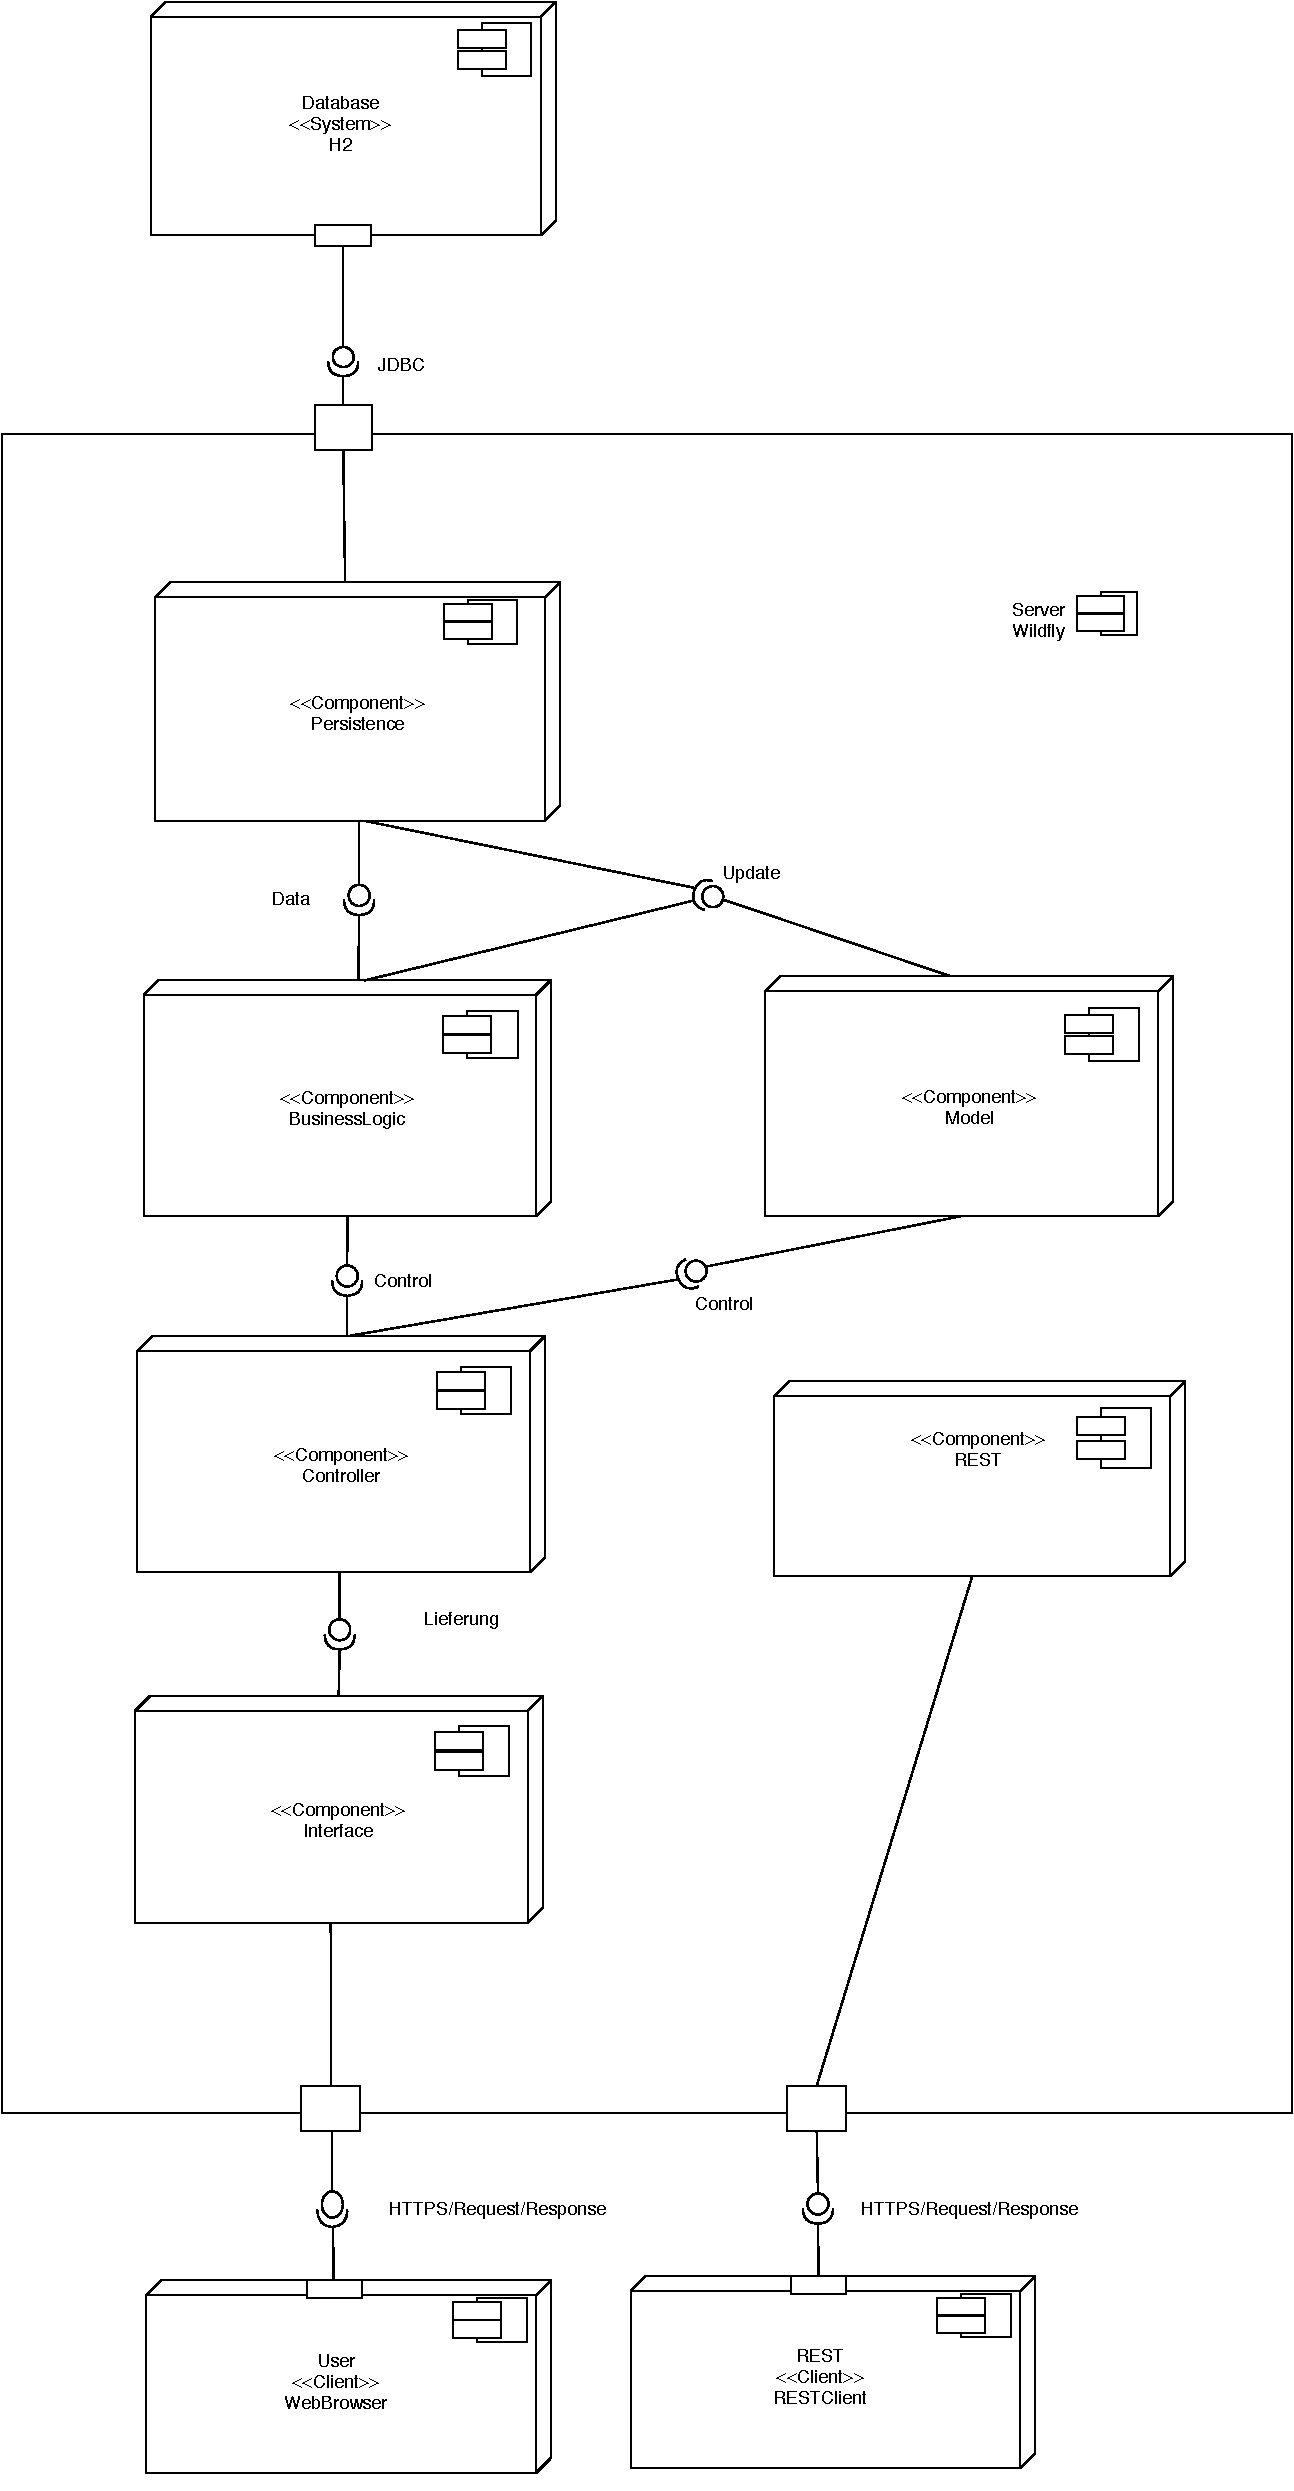
\includegraphics[width=340px]{UML/KonzeptioneleSicht.pdf}
  \caption{Die konzeptionelle Sicht}
  \label{fig:boat1}
\end{center}
\end{figure}
 

\section{Modulsicht}

\label{sec:modulsicht}
\begin{figure}[H]
\begin{center}
 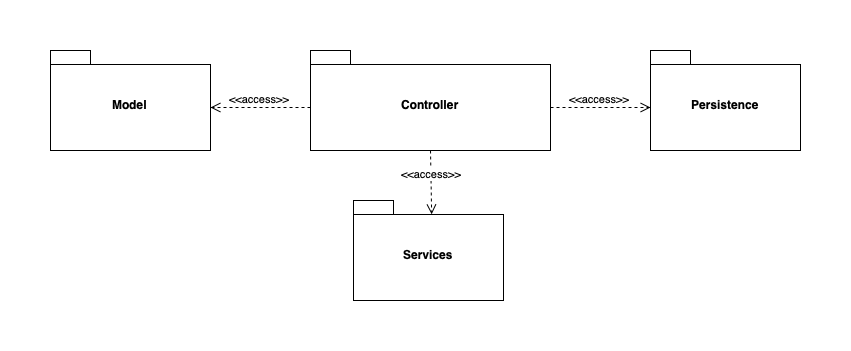
\includegraphics[width=310px]{UML/Modulsicht.png}
  \caption{Modul Sicht}
  \label{fig:boat1}
\end{center}
\end{figure}
\subsection{Pakete}

\subsubsection{Model}

\subsubsection{Controller}

\subsubsection{Persistence}

{
Die Persistenzklassen sind für die persistierung von Daten zuständig. Sie erben alle von der abstrakten Klasse ObjectDAO. Diese Klasse implementiert den EntityManager, der für das Verwalten der Datenbankinformationen zuständig ist. Die verschiedenen Funktionen sollen zum Beispiel das Speichern und das Laden nach einem Neustart von Daten ermöglichen. Jedes Objekt, was für die Speicherung in der Datenbank relevant ist, hat eine Klasse, die von ObjectDAO erbt. ObjectDAO hat drei abstrakte Funktionen, die jeweils in den Klassen für die einzelnen Objekte implementiert werden. Zusätzlich gibt es in zu jeder Klasse die relevanten Get Funktionen, um Informationen aus diesen Klassen zu bekommen. Die Funktion persist(T) speichert Objekte in die Datenbank. Update() überschreibt eine vorherige Version dieses Objektes mit der neuen und remove() entfernt das Objekt.

Hier wird das DAO-Pattern genutzt, wodurch die Programmlogik sich nicht an technische Deteils der Datenspeicherung halten muss. Datdurch ist ein flexibelerer Einsatz möglich. 
Dieses Paket wird gebraucht, da es vorgegeben ist. 
}

 \begin{sidewaysfigure}
  \caption{Persistenzmodelll für DataColorado}
  \centering
  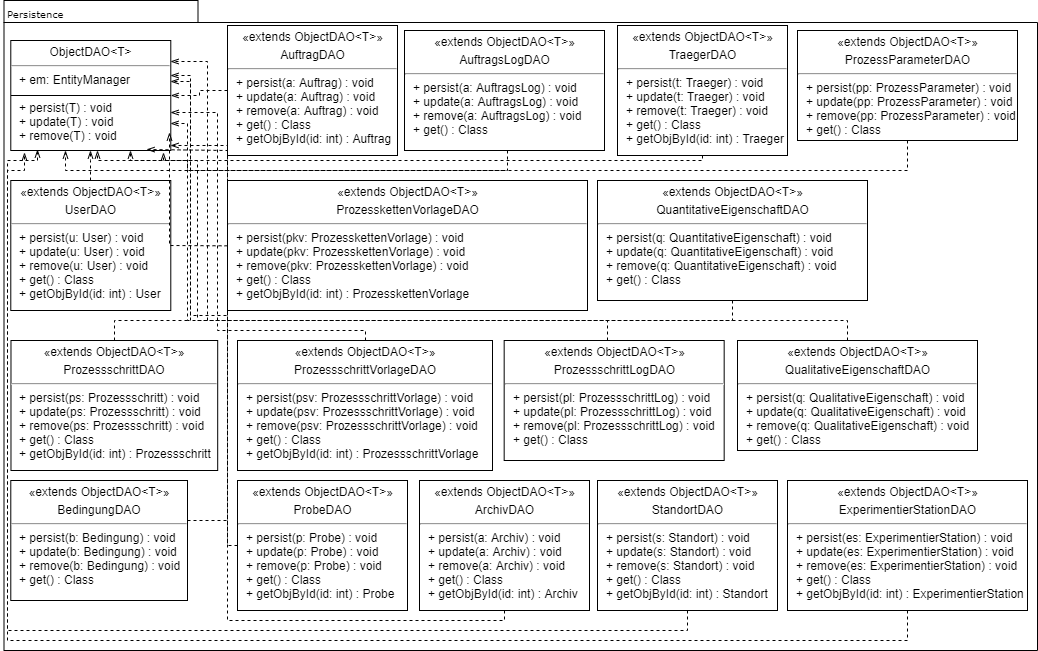
\includegraphics[width=\textwidth]{UML/Persistence}
 \end{sidewaysfigure}
 
\subsection{Services}
\begin{figure}[H]
\begin{center}
 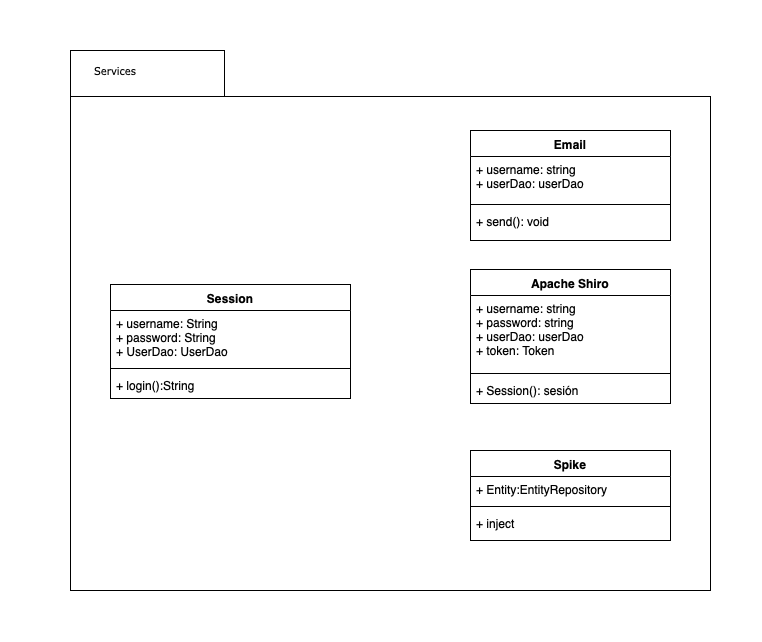
\includegraphics[width=310px]{UML/services.png}
  \caption{Services}
  \label{fig:boat1}
\end{center}
\end{figure}



\subsection{Module}



{\it
Diese Sicht beschreibt den statischen Aufbau des Systems mit Hilfe von
Modulen, Subsystemen, Schichten und Schnittstellen.
Diese Sicht ist hierarchisch, d.\,h. Module werden in Teilmodule
zerlegt. Die Zerlegung endet bei Modulen, die ein klar umrissenes
Arbeitspaket für eine Person darstellen und in einer Kalenderwoche
implementiert werden können. Die Modulbeschreibung der Blätter dieser
Hierarchie muss genau genug und ausreichend sein, um das Modul
implementieren zu können.

Die Modulsicht wird durch {UML}-Paket- und Klassendiagramme visualisiert.

Die Module werden durch ihre Schnittstellen beschrieben.
Die Schnittstelle eines Moduls $M$ ist die Menge aller Annahmen, die
andere Module über $M$ machen dürfen, bzw.\ jene Annahmen, die $M$
über seine verwendeten Module macht (bzw. seine Umgebung, wozu auch
Speicher, Laufzeit etc.\ gehören).
Konkrete Implementierungen dieser Schnittstellen sind das Geheimnis des Moduls
und können vom Programmierer festgelegt werden. Sie sollen hier
dementsprechend nicht beschrieben werden.

Die Diagramme der Modulsicht sollten die zur Schnittstelle gehörenden Methoden
enthalten. Die Beschreibung der einzelnen Methoden (im Sinne der Schnittstellenbeschreibung)
geschieht allerdings per Javadoc im zugehörigen Quelltext. Das bedeutet, dass Ihr
für alle Eure Module Klassen, Interfaces und Pakete erstellt und sie mit den Methoden der
Schnittstellen verseht. Natürlich noch ohne Methodenrümpfe bzw.\ mit minimalen Rümpfen.
Dieses Vorgehen vereinfacht den Schnittstellenentwurf und stellt Konsistenz sicher.

Jeder Schnittstelle liegt ein
Protokoll zugrunde. Das Protokoll beschreibt die Vor- und
Nachbedingungen der Schnittstellenelemente. Dazu gehören die erlaubten
Reihenfolgen, in denen Methoden der Schnittstelle aufgerufen werden
dürfen, sowie Annahmen über Eingabeparameter und Zusicherungen über
Ausgabeparameter. Das Protokoll von Modulen wird in der Modulsicht beschrieben.
Dort, wo es sinnvoll ist, sollte es mit Hilfe von Zustands- oder
Sequenzdiagrammen spezifiziert werden. Diese sind dann einzusetzen, wenn der
Text allein kein ausreichendes Verständnis vermittelt (insbesondere
bei komplexen oder nicht offensichtlichen Zusammenhängen).

Der Bezug zur konzeptionellen Sicht muss klar ersichtlich sein. Im
Zweifel sollte er explizit erklärt werden. Auch für diese Sicht muss
die Entstehung anhand der Strategien erläutert werden.
}




\section{Datensicht}
\label{sec:datensicht}

{

Alle Rollen die ein Nutzer annehmen kann, sind in einer Enum gepspeichert. Diese
sind TECHNOLOGE, PKADMIN, TRANSPORT, LOGISTIKER und der ADMIN. Hiermit
realisieren wir die Strategie 1.2 \ref{strategie:1.2}. Wir können somit mehrere Rollen für einen
User speichern. Um die Datensicherheit zu gewährleisten haben wir uns für
Apache Shiro entschieden. Hiermit können wir einzelnen Programmfunktionen nur
für bestimmte Rollen zulassen. Damit setzen wir die Strategie 2.1 \ref{strategie:2.1} um. Apache
Shiro muss wissen welche Rollen zu welchen Usern gehören. Daher referenziert
User eine oder mehrere Rollen.


Die User bestehen aus einer id, einem Vornamen, einem Nachnamen, einer Email,
einer Telefonnummer, einer Kombination von seinem Passwort und seinem Usernamen.
Der User erhält nach dem sein Konto erstellt wurde eine email, nachdem er seinen
Account verifiziert, wird wurdeVerifiziert auf True gesetzt. Das Attribut
Erstellungsdatum, speichert wann der Nutzer erstellt worden ist.

Ein Standort enthält ein String in dem der Ort des Standorts steht.

Ein Träger hat eine id, einen Standort. Falls er einem Auftrag zugewiesen ist,
referenziert er auch diesen.

Es gibt standardmässig die Trägerarten eingebettet, einzelnen und Glas. Diese sind in
der Klasse Trägerart gespeichert. Die Information über die Trägerarten wird
benötigt um in Erfahrung zu bringen, ob eine Experimentierstationen ein
ProzessSchritt ausführen kann. Die ProzessSchrittVorlage hat als Attribut welche
Träger sie annimmt und welche Träger sie ausgibt (eingabeTräger. ausgabeTräger).
Siehe Strategie 17.3 \ref{strategie:17.3}.

Wir haben das Archiv als eigenständig Klasse modelliert, so können wir im
Nachhinein Proben, welche archiviert werden eine Referenz zu einer Instanz von
Archiv geben. Falls es diese Referenz gibt, so können wir wissen, dass diese
Probe Archiviert wurde. Dies wird in der Strategie 16.1 \ref{strategie:16.1} umgesetzt

Es gibt Zwei Arten von Eigenschaften die wir modellieren. Die Qualitative
Eigenschaft beschreibt ob das Objekt diese Eigenschaft hat. Sie hat also ein
Namen, falls es eine Referenz dahin gibt, wissen wir dass das Objekt auch diese
Eigenschaft hat. Die Quantitative Eigenschaft ist eine Erweiterung der
Qualitativen Eigenschaft. Sie enthält einen Wert und eine Einheit. Der Wert ist
eine Zahl, welche von Java unterstützt wird. Für die Einheiten nutzen wir die SI
Implementierung, welche die Java Laufzeit Bibliothek bereitstellt. Dies
ermöglicht es unserem System mit Eigenschaften und Anforderungen umgehen zu
können. Es ist uns hiermit möglich, Proben mit spezifizierten Eigenschaften zu
finden und diese dann bestimmten Klassen zuzuweisen. Für Experimentierstationen gelten
Bedingungen, diese werden durch Eigenschaften oder Prozess-Parametern realisiert.
Wir können festlegen, dass ein Prozesschritt nur ausgeführt werden kann, wenn
ein vorheriger Prozesschritt eine Eigenschaft besitzt oder ein Parameter hat.
Ein Logistiker kann in der Logistik Ansicht Proben auflisten, welche
einer Bedingung entsprechen. Hier haben wir die Strategie 10.2 \ref{strategie:10.2} umgesetzt.

Eine ProzesschrittVorlage, enthält eine eindeutige ID, einen Zustandsautomaten
(ProzessSchrittZustand) und die geschätzte Dauer für den ProzessSchritt.
Strategie 19.2 \ref{strategie:19.2}  setzen wir um, indem wir die Zustände einer ProzessSchrittVorlage
nicht als Enum speichern, sondern sie als Klasse modellieren.
Das Attribut eingabeTräger ist Liste von Trägerarten die als Eingabe akzeptiert
werden, die Liste der Trägerarten ausgabeTräger beschreibt welche Träger von
diesem Prozesschritt ausgeben werden.

Die enum AuftragsPriorität enthält die Prioritäten, welche eine Prozesskette
haben kann. Falls ein Prozesschritt eine höhere Priorität hat, wird dieser vor
dem Prozesschritt ausgeführt der eine geringere Priorität hat.  Somit kann dann
automatisch bestimmt werden, welcher ProzessSchritt als nächstes an einer
Experimentierstation ausgeführt wird unter Berücksichtigung der Priorität.
Hiermit setzen wir die Strategie 7.2 \ref{strategie:7.2}  um.

Es gibt drei Arten von ProzessSchrittArten: umformend, färbend und ermittelend.
Diese wurden als Enum modeliert, dies ist unsere Umsetzung der Strategie 20.1 \ref{strategie:20.1} 
Diese sind vom Kunden Vorgeben und können nicht im Nachhinein geändert werden.

Ein ProzessSchritt ist eine instanzierte ProzesschrittVorlage. Ihre Attribute
sind, eine Prozesschritt ID, ein Boolean uploaded. Dieser wird auf True gesetzt,
nachdem der Technologe die ProzessParameter an die externe Datenbank hochgeladen
hat. current ist referiert eine Experimentierstation, falls es eine
Experimentierstation gibt, wo aktuell dieser Prozesschritt durchläuft. Der
Aktuelle Zustand aus dem Zustandsautomaten des Prozesschrittes wird in dem
String Zustand gespeichert. TODO Warum hat PS einen Auftrag

Ein ProzessSchrittZustand ist eine Liste von Zuständen. Der
ProzessSchrittZustand kann vom pkAdmin erweitert um weitere Zustände erweitert
werden, wenn dieser nicht in Benutzung ist.

Ein ProzessParameter hat einen Namen. Einer ProzesschrittVorlage Vorlage können
Parameter zugewiesen werden. Bei falls der Prozesschritt ermittelnd ist, wird
nachher die Eigenschaft, welche ermittelt wurde der Probe zugewiesen.

Um den Up/Download von den Parameter der Prozesschritte als JSON zu ermöglichen
ist es diese mit JAXB zu serialisieren. Dazu verwenden wir
TODO. Hiermit setzen wir die Strategie 4.1 \ref{strategie:4.1}  um. Dafür stellen wir ein Interface
bereit, dass es uns ermöglicht die Parameter der Prozesschritte zu serialiseren.
Um mit externen Diensten zu kommunizieren werden für das serialisierte JSON
Rest-Schnittstellen angeboten

Eine ProzesskettenVorlage, hat eine eindeutige id. Aufträge besitzen
Prioritäten. AuftragsPriorität ist bei uns eine Enum. Die Prioritäten sind fest
und können im Nachhinein nicht mehr geändert werden.


Die Enum ProzesskettenZustandsautomat enthällt alle Zustände die eine Auftrag
haben kann. Diese sind fest und können im nachhinein nicht mehr geändert werden.
Deshalb werden sie als Enum gespeichert. Hiermit wird die Strategie 18.1 umgesetzt.

Ein Auftrag ist eine Instanz einer Prozesskettenvorlage.

Wie oben erwähnt ist Auftrag eine Instanzierung von der Prozesskette, die
ProzesschrittVorlage erstellt eine ProzessSchritt Objekt. Wir haben getrennte
Klassen für die Vorlage und die Instanzen von den Prozesschritten und Prozessketten.
Hiermit setzen wir die Strategie 3.1 \ref{strategie:3.1}  um. Die ProzessSchritte sind somit abstrakt
und können später auch in anderen Prozessketten wiederverwendet werden.

Ein AuftragsLog enthält start und end Zeiten für die instanzierte Prozesskette.
Diese Referentiert auch alle Prozesschritlogs welche in dem Auftrag enthalten
sind. Aus diesen ist zu entnehmen, wann der einzelne Prozesschritt gestartet
worden ist, in welchem Zustand dieser sich befand und wann er beendet worden
ist. Falls später dann ein Prozesschritt betrachtet wird, enthält er die Logs
und seine Prozesschritt Parameter. Die ProzessSchrittparameter lassen sich zu
JSON serialisieren (Strategie 4.1) \ref{strategie:4.1} , der ProzesschrittLog sowie der Prozesschritt
ansich sind auch serialisierbar. Jetzt ist es uns möglich ein Protokol
der Prozesskette zu serialisieren.


Eine Experimentierstation besteht aus einer eindeutig ID, einem Standort, der
als String gespeichert wird sowie einer Enum die den Status der Station
enthält. Jede der Experimentierstationen enthält eine Warteschlange, welche alle
Prozesschritt Instanzen enthält, welche auf die Durchführung an dieser Station
warten. Um in einer in die Warteschlange zugewiesen zu werden muss unser System
folgendes tun. Einer ProzesschrittVorlage können Bedingungen hinzugefügt werden,
ein Beispiel wäre die Existenz einer Wärmebehandlung. Experimentierstationen
können auch Parameter oder Eigenschaften zugewiesen werden.
Aus dem Bedingungen der ProzesschrittVorlage ergibt sich die Menge an
Experimentierstationen, welche möglich sind. Für diese wird geschätzt, wie lange
es dauert bis die bisherige Warteschlange beendet ist. Die Experimentierstation
mit der geringsten Wartezeit wird dem Prozesschritt zugeteilt. Dies ist unsere
Umsetzung von der Strategie 14.2 \ref{strategie:14.2} .

Zu einer Station können mehrere User vom Administrator zugewiesen
werden. User, welche der Station zugeordnet sind haben die Möglichkeit den
Zustand der Station zu erfragen und zu verändern. Hiermit wir die Strategie 6.1
umgesetzt. Um diese Änderungen zu Persistieren Nutzen wir Deltaspike Data. Dafür
müssen wir einen EntityManager konfigurieren, der über CDI injected wird. Dies
können wir mit dem EntityManagerProducer umsetzen. Für die Experimentierstation
erstellen wir nun eine Repository Klasse. Mit der Querry Annotation ist es uns
nun möglich SQL ähnliche Queries für unsere modellierten Klassen zu erstllen

Jede der Proben enthält eine eindeutige ID, diese entspricht dem ID Schema,
welches der Kunde schon in seiner jetzigen Datenbank nutzt. Kommentare und deren
Zeitstempel werden als Pair gespeichert (Strategie 21.3)\ref{strategie:21.3}  und von den
Useren bearbeitet. Somit kann jede Probe in dem System betrachtet werden.
Dadurch, dass wir für jede Probe eine ID haben und sie einzeln in der Datenbank
speichern wird Strategie 8.1 \ref{strategie:8.1} umgesetzt. Somit kann nachvollzogen werden, zu
welchem Zeitpunkt sich eine Probbe wo und in welcher Prozessketten befunden hat.
Weiter kann der Technologe durch das kommentieren einzelner Proben wichtige
Informationen über eine Probe an seine Mitarbeiter weitergeben. Damit die Nutzer
der Proben Verwaltung nicht unter langen Ladezeiten leiden, laden wir nur Proben
aus der Datenbank, welche wir auch benötigen. Dies wird durch deltaspike data
und einem Query, der nur einen kleinen Ausschnitt aus der Datenbank lädt,
realisiert. Wir nutzen also lazy loading und setzen damit die Strategie 12.1 \ref{strategie:12.1} um.

Ein Träger enthält Referenzen zu alle Proben die in Ihm enthalten sind. Weiter
hat der Träger ein Standort und eine ID. Träger ist eine assoziations Klasse von
Auftrag und Prozesschritt (TOOD Warum Leo). Falls der Zustand eines
Prozesschrittes sich verändert und Proben zwischen Experimentierstationen
transportiert werden sollen, weisen wir ein Träger, falls nötig, dem neuen
Schritt zu und setzen alle Proben in den Träger. Das Ziel, der aktueller
Standort, die Proben und deren Träger können dann dem Transport als neuem
Transport Auftrag zugewiesen werden. Der Transportauftrag ergibt sich impliziert
aus dem Auftrag. Er wird dadurch realisiert, dass ein Transporteur nur die für
ihn relevanten Informationen erhält.

Falls ein Prozesschritt ein Transport Auftrag den Zustand freigeben hat, wird er
allen Transportern angezeigt. Wenn er Transporteur diesen annimmt, wird der
AuftragsZustand auf angenommen gesetzt. Jetzt verschwindet der Auftrag auch für
die anderen Transporteure in der Transort Ansicht. Der Transporteur läuft nun
los und erledigt den Auftrag, danach wird der AuftragsZustand auf abgegeben
gesetzt. Der Transport erfährt in seiner Ansicht, wo die Proben sich befinden
und was ihr nächstes Ziel ist. Er selber wird nicht persistiert. Dies ist unsere
Umsetzung von der Strategie 13.1 \ref{strategie:13.1} 




  . Eine bestimmte Probe kann ausschließlich einem Träger zugeordnet werden.
{\it Hier wird das der Anwendung zugrundeliegende Datenmodell
  beschrieben. Hierzu werden neben einem erläuternden Text auch ein
  oder mehrere {UML}-Klassendiagramme verwendet. Das hier beschriebene
  Datenmodell wird u.\,a. jenes der Anforderungsspezifikation enthalten,
  allerdings mit implementierungsspezifischen Änderungen und
  Erweiterungen. Siehe die gesonderten Hinweise.}
   
 \begin{sidewaysfigure}
   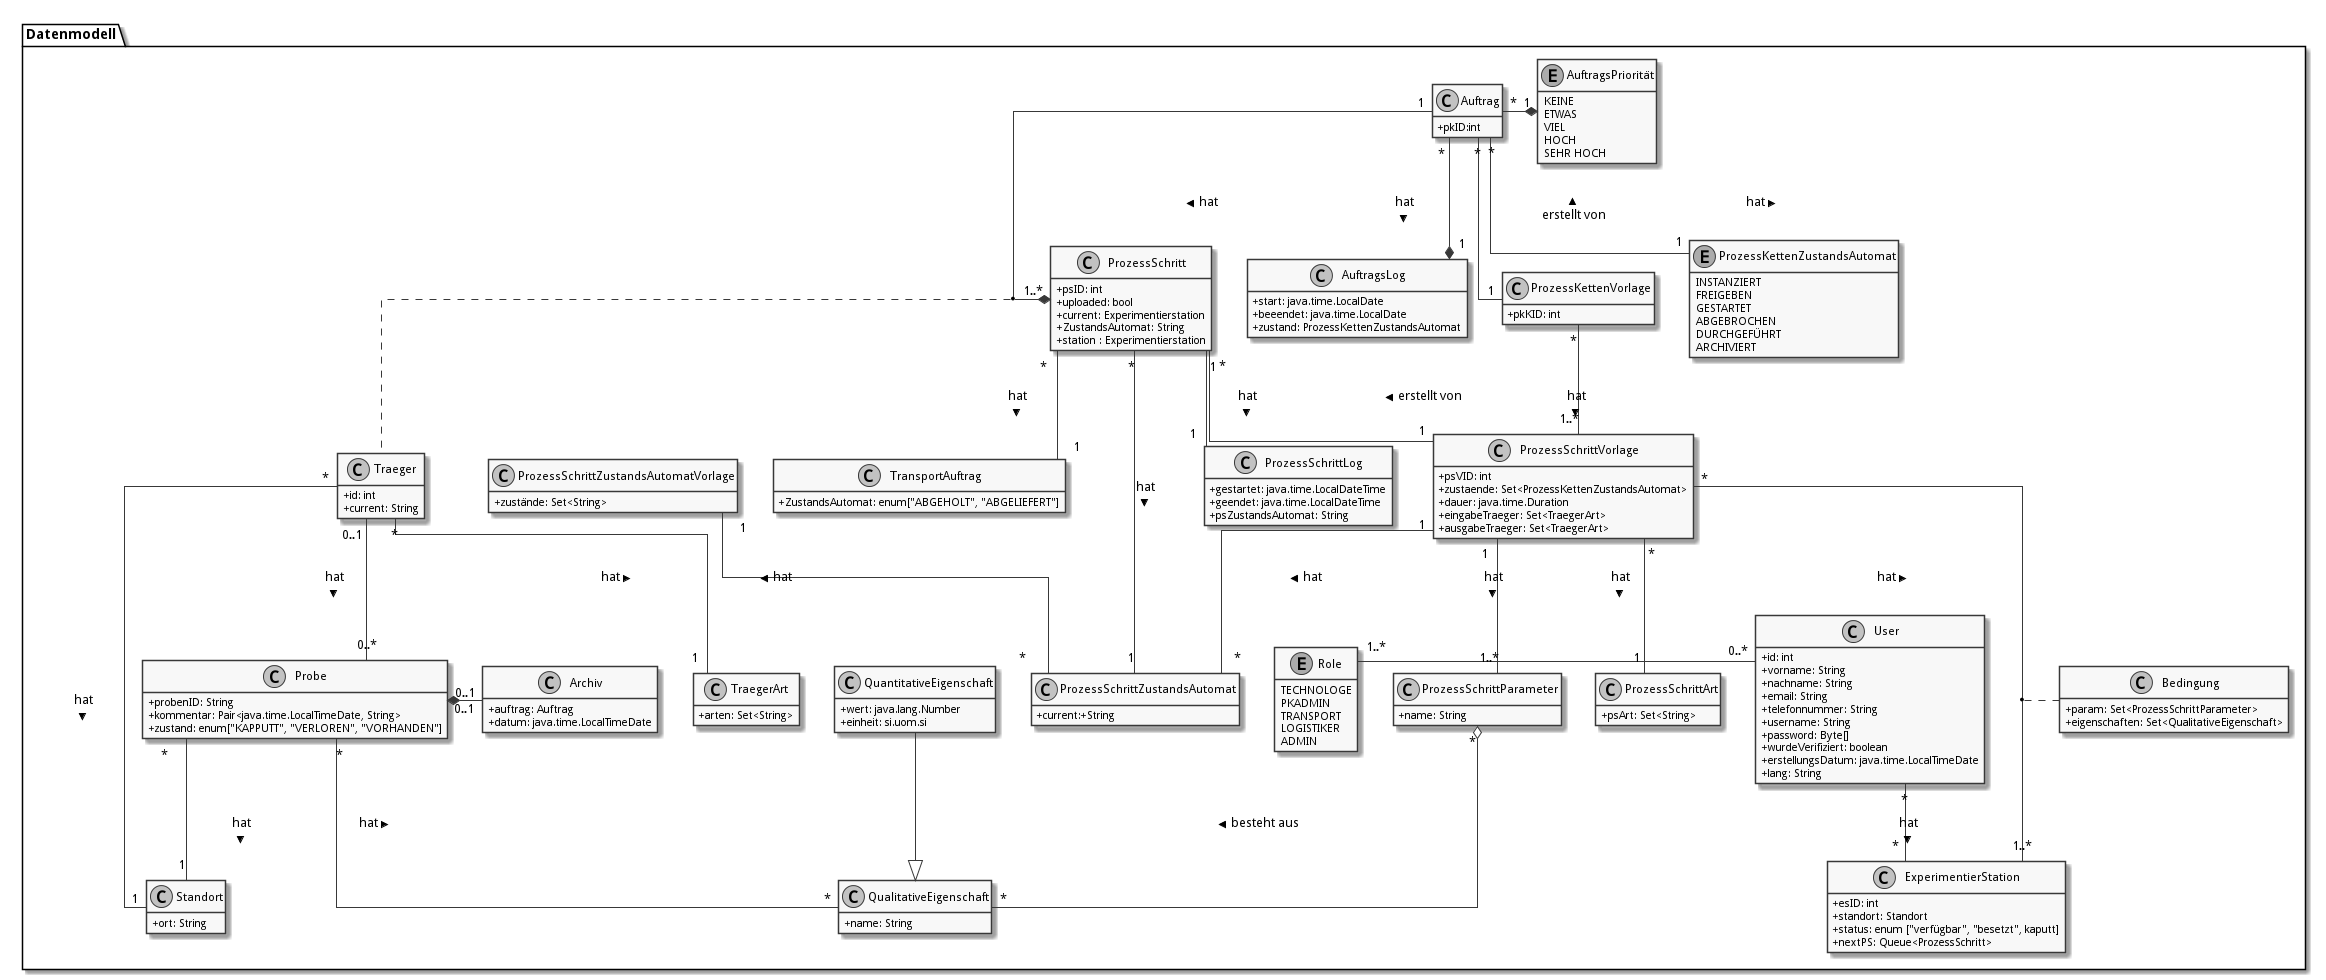
\includegraphics[width=\textwidth]{UML/datenModel}
  \caption{Datenmodell für DataColorado}
  \centering
 

 \end{sidewaysfigure}
\newpage
\section{Ausführungssicht}

\label{sec:ausfuehrung}


{ Im folgenden Schritt werden wir die Ausführungssicht erläutern. Es wird aufgezeigt, welche verschiedenen Geräte benötigt werden, welche Prozesse auf den Geräten jeweils laufen und welche Module dort enthalten sind.
}


%%\includepdf[]{06Ausfuehrungssicht.pdf}
\begin{figure}[H]
\includegraphics[scale=0.5]{UML/06Ausfuehrungssicht.pdf}
 \caption{Ausführungssicht}
\end{figure}


{ Die Ausführungssicht von unserer Software (SWP2) ist in der obigen Abbildung
  7.1 modelliert.

Beliebig viele Benutzer können via TCP/IP auf den SFB-Server zugreifen. Dies
geschieht über eine Webapplikation, die im Internetbrowser eines PCs oder eines
mobilen Endgeräts aufgerufen werden kann.

Es ist auch möglich, dass ein Rest-Client sich mit unserem Server verbindet,
dieser verbindet sich dann an den REST-Endpunkt über den SFB-Server. Das Modul
der Businesslogik führt die Befehle dann aus.

Es gibt einen Anwendungsserver, welchen wir SFB-Server genannt haben, auf dem
eine Instanz von Wildfly läuft. Auf dieser Wildflyinstanz wird der SWP2-Server
mit allen dazugehörigen Modulen ausgeführt.

Das Modul Persistence kommuniziert mit dem Modul Businesslogik aber auch
\glqq abstract\grqq{} über JDBC mit dem H2 Server.

Der SFB-Server stellt eine Verbindung über TCP/IP zu der
Datenbank her, welche auf dem gleichen SFB Server läuft und eine Instanz der Datenbanksoftware H2 betreibt.
}

\section[Zusammenhänge zwischen Anwendungsfällen und Architektur]{Zusammenhänge zwischen Anwendungsfällen und Architektur\sectionmark{Zusammenhänge AF u. Architektur}}
\sectionmark{Zusammenhänge AF u. Architektur}
\label{sec:anwendungsfaelle}


\subsection{Login eines Benutzers}
\begin{figure}[H]
  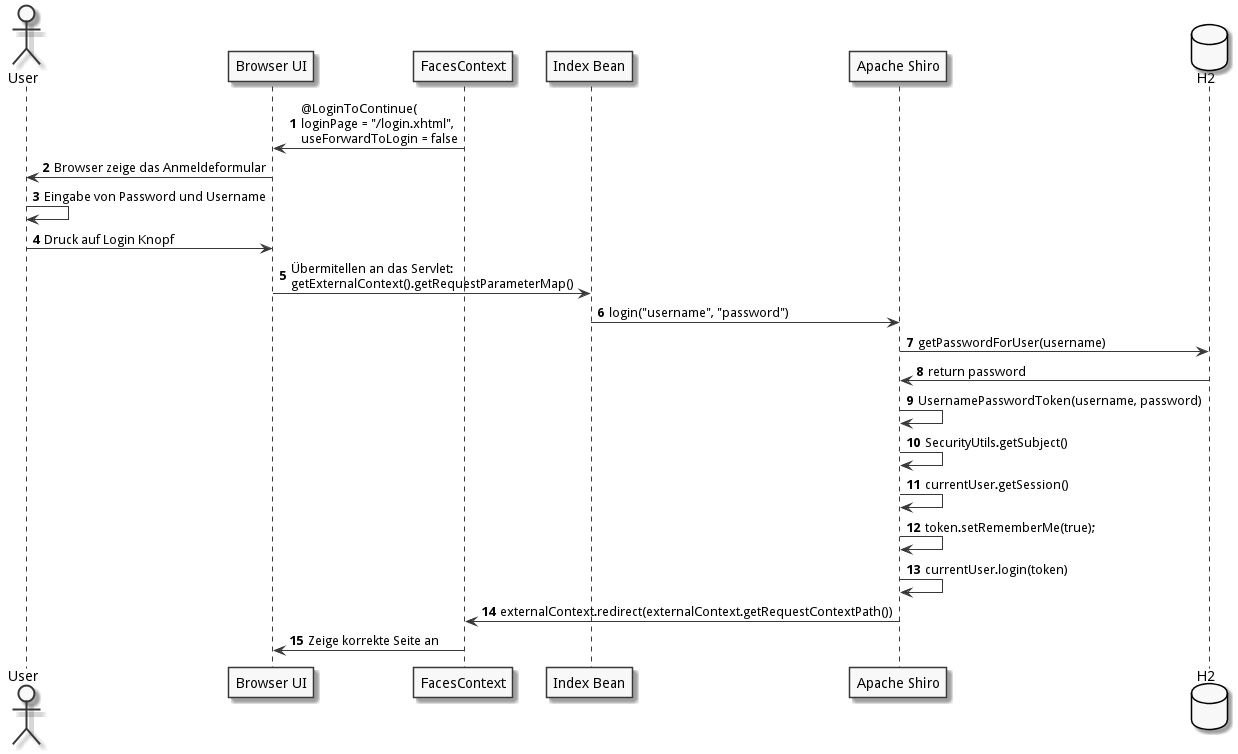
\includegraphics[width=\linewidth]{UML/aw/erstbenutzung.png}
  \caption{Sequenzdiagrammen des Loginvorganges}
  \label{fig:erstbenutzung.png}
\end{figure}

In diesem Anwendungsfall geht es darum zu zeigen, was passiert wenn sich ein
Benutzer anmeldet. Wir haben uns entschieden, die Sichehheite nicht selber zu
implementieren, sondern Apache Shiro zu nutzen \ref{problemkarteXXX}

\subsection{Was ist Apache Shiro}
Als erstes möchten wir einen überblick über Apache Shiro geben, als dann wird Anhand
des Sequenzdiagrammes erläutert, wie Apache Shiro mit unseren Schichten
zusammenhängt. Apache Shiro kann ab jetzt auch nur als Shiro bezeichnet werden.

Shiro ist ein sehr mächtiges und leistungsstarkes Java Security Framework,
welches sich das Ziel gesetzt hat Entwicklern eine intuitive jedoch auch
umfassende Lösung für Authentifizierung, Autorisierung und Session-Management zu
bieten. Shiro basiert auf einem soliden, Schnittstellengesteuerten Design und
folgt OO-Prinzipien.

Ein \emph{Subject} ist eine sicherheitsspezifische Sicht auf einen Nutzer
unseres Programms. Dabei wird nicht zwischen einem menschlichen Nutzer und
einem maschinellen unterschieden. Auch in der Sicherheitswelt ist der Begriff
Subject eigentlich die anerkannte Nomenklatur. Die Session erlaubt es dem
Nutzer bestimmte Operationen durchzuführen. Es ist weiter möglich einer Session
weitere Attribute zu geben. Unsere Session ist eine Shiro-spezifische Instanz,
welche das meiste bietet davon bietet,  was uns auch eine reguläre HttpSession
bietet. Der Vorteil der Session ist es, dass sie keine HTTP-Umgebung braucht.

Bei uns wird die Session in einer Webapplikation umgesetzt, folglich basiert
unsere Session auf die standardmäßige HttpSession.

Wir haben uns für ein rollenbasiertes Zugriffssystem entschieden. TODO
Strategie. Um dies in Shiro umzusetzen, benutzen wir das von Shiro bereitgestellte
JdbcRealm. Mit JdbcRealm kann Shiro aus unserer Datenbank die benötigen
Attribute und Rollen eines Nutzers laden

\subsection{Erklärung des Diagramms}
Es kann vorkommen, dass ein Benutzer unseres Systems in einen Realm navigiert,
der nur für bestimmte Rollen zugänglich ist \textbf{Schritt 1} Dies ist der Fall
für den ersten Schritt unseres Sequenz Diagrammes. Dies passiert in einem
FacesContext. Der Webbrowser auf die $login.xhml$ weitergeleitet. Dort erscheint
ein Login Formular \textbf{Schritt 2}, in dem der Nutzer seine Anmeldedaten
eingeben kann \textbf{Schritt 3}. Das Formular wird vom Browser an unseren
Server gesendet \textbf{Schritt 4}. Für die spätere Verarbeitung brauchen wir
wir die Parameter die es in dem Kontext der Anmeldung gab. Diese werden in
\textbf{Schritt 5} an das Login Bean gesendet. Das Login Bean hat die Aufgabe
weitere Sichheitsfunktion an Shiro zu delegieren. Dafür nutzen die Methode login
Methode der IndexBean. Die hat die Aufgabe zu ermitteln in welchem Kontext die
Login anfrage gestellt wurde. Sobald dies ermittelt wurde ruft sie delegiert sie
weiter an Shiro. \textbf{Schritt 6}. Um das Passwort aus der Datenbank zu lesen,
nutzen die von Shiro bereitgestellte Methode \textbf{Schritt 7}. Die Datenbank
liefert uns dann das Passwort. In diesem Sequenzdiagramm wurde abstrahiert, dass
Passwörter gehashed und gesalted werden. Dies liegt daran, dass Shiro, falls so
konfiguriert dies im Hintergrund macht.

Shiro verlangt für ein Token für den Login. Der Token wird aus dem Passwort
und dem Benutzernamen generiert. das genierierte Token hat den Datentyp
UserNameToken.  Das Token wir in  Schritt \textbf{Schritt 9} generiert.


Ein schon angemeldet Nutzer, kann sich nicht nochmal anmelden. Daher müssen wir
überprüfen ob unser Subject anonym ist \textbf{Schritt 10}.

Subjects können Sessions besitzen. Shiro holt und merkt sich die Session eines
Subjects in \textbf{Schritt 11 \& 12}. So haben wir nun ein Subject und seine Session.
Hiermit können wir nützliche Dinge tun. Beispielsweise überprüfen, ob das
Subject die die benötigte Rolle hat. Unsere obige Subject Instanz repräsentiert
den akutellen Nutzer, aktuell ist unser Subject aber noch anonym. Um nicht mehr
anonym zu sein muss sich ein Subject anmelden. Für den Anmeldeschritt führen wir
ein Login mit unserem Token auf unserem aktuellen Nutzer aus \textbf{Schritt
  13}. Nach der erfolgreichem Authentifizierung leiten wir den Nutzer auf den
ursprünglichen zurück.  \textbf{Scrhitt 14}. Dafür Verwenden dafür nutzen wir
eine Weiterleitung die den Pfad zu dem FacesContext kennt, die Anmeldung
gefordert hat.

\subsection{Kleiner Auschschnitt zur Fehlerbehandlung}
Bei dem Login können folgende Exceptions geworfen werden:
\begin{itemize}
  \item Shiro löst eine UnknownAccountException aus, falls es den Nutzer nicht gibt
  \item Shiro löst eine IncorrectCredentalException aus, falls das Token nicht
  stimmt
  \item Falls das Konto des Users gesperrt ist. Wird ein LockedAccountException
  ausgelöst.
\end{itemize}

\subsection{Prozessketten Verwalten und Proben beantragen}

\begin{figure}[H]
  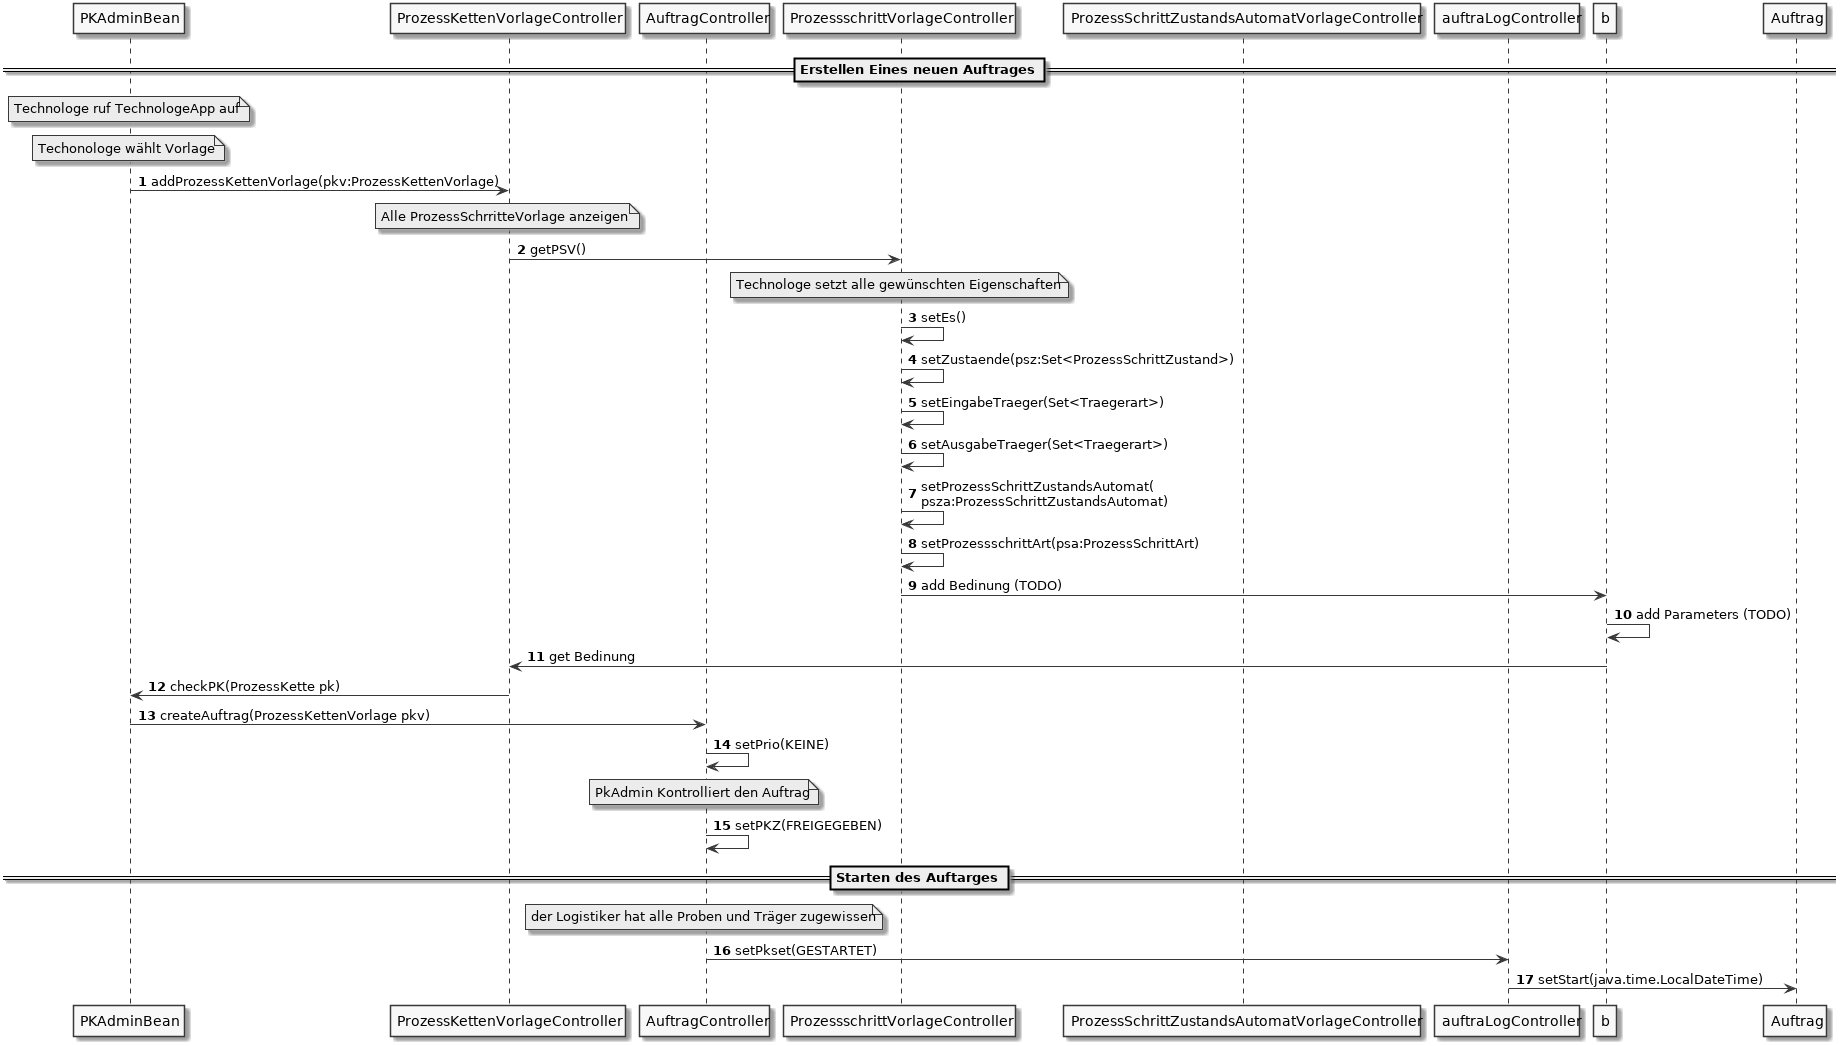
\includegraphics[width=\linewidth]{UML/aw/erstellepk.png}
  \caption{Ablauf des Erstellens einer Prozesskette}
  \label{fig:pkErstellen}
\end{figure}

Figure \ref{fig:pkErstellen} zeigt wie der Prozesskettenadministrator die Prozesskette erstellt. 
Bei Schritt 18, schauen sie bitte in Graphik \ref{fig:logstikProbenPüftZuweisen}. 

Der Prozesskettenadministrator wählt aus den vorhandenen Vorlagen eine aus, damit erstellt er einen neuen Auftrag und legt für diese alle Parameter fest.
Falls die Randbedingen der Kette stimmen darf diese instanziiert werden. Beim Speichern des Auftrages mit der instanzierten Prozesskette werden diese auch persistiert.

Jetzt erhält der Logistiker einen neuen Probenzuweisung Auftrag, falls die Anfrage genehmigt wurde kann der PKAdmin nun die Prozesskette starten


%In der Graphik \ref{fig:logstikProbenPüftZuweisen} erhält die Logistik eine Anfrage für die Probenverwaltung. Es muss nun vom System geprüft werden ob %Proben mit den gewünschten Materialeigenschaften im Lager sind. Das System gibt diese an die Logistik zurück. Werden die Proben dann von dem %Logistiker ausgewählt und genehmigt, so werden diese an den Auftrag übermittelt und persistiert. Die Genehmigung wird an die Prozesskettenverwaltungs-%Administrationsapp übermittelt.


\subsection{ProzessSchritt Sequenzdiagramm}




{\it In diesem Abschnitt sollen Sequenzdiagramme mit Beschreibung(!)
  für zwei bis drei von Euch ausgewählte
    Anwendungsfälle
  erstellt werden. Ein Sequenzdiagramm beschreibt den
  Nachrichtenverkehr zwischen allen Modulen, die an der Realisierung
  des Anwendungsfalles beteiligt sind.  Wählt die
    Anwendungsfälle so, dass nach Möglichkeit alle Module Eures
    entworfenen Systems in mindestens einem Sequenzdiagramm
    vorkommen. Falls Euch das nicht gelingt, versucht möglichst viele
    und die wichtigsten Module abzudecken. }

\section{Evolution}

\label{sec:evolution}
Um die Anwendung nach der Auslieferung an den Kunden entwickel- und erweiterbar zu halten, wird die Software in verschiedene Module aufgeteilt und eine gute Entkopplung \& Kapselung dieser kommen der Erweiterung der Software zugute. Im Folgenden präsentieren wir Ideen zur Erweiterung der Software.

\subsection{Automatische statistische Auswertung} 
{ Die erste Idee zum
  sinnvollen Erweitern der Software soll eine Voraussicht ausgeben können, wie
  sich nach dem Ausführen eines beliebigen ProzessSchritts auf eine Probe ihre
  Eigenschaften ändern würden, bzw. welche Eigenschaften die Probe danach
  wahrscheinlich haben wird. Da wir in der Datenbank ca. eine halbe Million
  Proben haben, kann ein analytischer Algorithmus Statistiken erstellen, welche
  die höchste Wahrscheinlichkeit einer Veränderung der Eigenschaften einer Probe
  auswertet. Um es in unsere Architektur einzubinden, muss eine Klasse für die
  Statistiksoftware erstellt werden, aus dieser werden die Statistiken erstellt
  und dann mit den eingegebenen Daten abgeglichen. Am Ende bekommt man die
  Änderung der Eigenschaften zurück, die am wahrscheinlichsten ist, wenn ein ProzessSchritt auf die Probe angewandt wird.
}
\subsection{Voraussichtliche Dauer eines Prozesses} 
{ Man kann den Algorithmus aus der automatischen statistischen Auswertung auch dafür verwenden, dass aus den durch den Algorithmus aus 9.1 errechneten empirischen Daten die voraussichtliche Dauer eines Prozesses errechnet und ausgegeben wird. Hier braucht man, wie in 9.1, eine neue Klasse, welche die Statistiksoftware beinhaltet, aus welcher man dann eine wahrscheinliche Zeit herausbekommt.
}
\subsection{Scanner}{
  Da so gut wie jedes mobile Endgerät eine Kamera besitzt, könnte man diese nutzen, um QR-Codes, die auf den Proben, den Trägern, im Archiv und an jeder Station zu finden sind, zu scannen damit z. B. der Transporter nicht mehr manuell eingeben muss, welche Datei er wohin bringt. \\
  Er scannt den QR-Code des Trägers und dann die QR-Codes beliebig vieler
  Proben. Die Software ordnet nun automatisch die gescannten Proben dem
  gescannten Träger zu.
  Er kann den QR-Code des Trägers scannen und die Software weiß automatisch,
  dass der angemeldete Transporter den Träger abgeholt hat und wenn er jetzt den
  QR-Code der nächsten Experimentierstation scannt, trägt die Software
  automatisch den Träger als abgeliefert ein. \\

  Um dies zu realisieren, muss die REST-API so erweitert werden, dass über
  die Businesslogik die Proben und Träger im Modell aktualisiert werden. Der
  Zustand der jeweiligen ProzessSchritte muss ebenfalls verändert werden.
}



\end{document}


%%% Local Variables:
%%% mode: latex
%%% mode: reftex
%%% mode: flyspell
%%% ispell-local-dictionary: "de_DE"
%%% TeX-master: t
%%% End:
